\documentclass[onecolumn, draftclsnofoot,10pt, compsoc]{IEEEtran}
\usepackage{graphicx}
\usepackage{url}
\usepackage{setspace}
\usepackage[font=small,labelfont=bf]{caption} % Required for specifying captions to tables and figures
\usepackage[final]{pdfpages}
\usepackage{tabularx}
\usepackage{geometry}
\geometry{textheight=9.5in, textwidth=7in}

% 1. Fill in these details
\def \CapstoneTeamName{		Malsano}
\def \CapstoneTeamNumber{		72}
\def \GroupMemberOne{			Brandon Jolly}
\def \GroupMemberTwo{			Katherine Jeffrey}
\def \GroupMemberThree{			Bradford Wong}
\def \CapstoneProjectName{		App to Support Field Diagnostics in Veterinary Medicine}
\def \CapstoneSponsorCompany{	Oregon Veterinary Diagnostic Laboratory}
\def \CapstoneSponsorPerson{		Dr. Christiane Loehr}

% 2. Uncomment the appropriate line below so that the document type works
\def \DocType{		%Problem Statement
				Project Hand Off
				%Technology Review
				%Design Document
				%Progress Report
				}
			
\newcommand{\NameSigPair}[1]{\par
\makebox[2.75in][r]{#1} \hfil 	\makebox[3.25in]{\makebox[2.25in]{\hrulefill} \hfill		\makebox[.75in]{\hrulefill}}
\par\vspace{-12pt} \textit{\tiny\noindent
\makebox[2.75in]{} \hfil		\makebox[3.25in]{\makebox[2.25in][r]{Signature} \hfill	\makebox[.75in][r]{Date}}}}
%3. If the document is not to be signed, uncomment the RENEWcommand below
%\renewcommand{\NameSigPair}[1]{#1}

%%%%%%%%%%%%%%%%%%%%%%%%%%%%%%%%%%%%%%%
\begin{document}
\begin{titlepage}
    \pagenumbering{gobble}
    \begin{singlespace}
    	
\includegraphics[height=4cm]{coe_v_spot1}
        \hfill 
        % 4. If you have a logo, use this includegraphics command to put it on the coversheet.
        %\includegraphics[height=4cm]{CompanyLogo}   
        \par\vspace{.2in}
        \centering
        \scshape{
            \huge CS Capstone \DocType \par
            {\large\today}\par
            \vspace{.5in}
            \textbf{\Huge\CapstoneProjectName}\par
            \vfill
            {\large Prepared for}\par
            \Huge \CapstoneSponsorCompany\par
            \vspace{5pt}
            {\Large\NameSigPair{\CapstoneSponsorPerson}\par}
            {\large Prepared by }\par
            Group\CapstoneTeamNumber\par
            % 5. comment out the line below this one if you do not wish to name your team
           \CapstoneTeamName\par 
            \vspace{5pt}
            {\Large
                \NameSigPair{\GroupMemberOne}\par
                \NameSigPair{\GroupMemberTwo}\par
                \NameSigPair{\GroupMemberThree}\par
            }
            \vspace{20pt}
        }
        \begin{abstract}
        % 6. Fill in your abstract    
Currently, there are many difficulties for veterinary pathologists trying to perform remote diagnostics. There are not any effective ways for people out in the field collecting samples to communicate with specialized experts located in laboratories. As a result, this project will involve creating an Android mobile application that will be used as a bridge to connect the field personnel with the veterinary pathologists in laboratories. With this mobile application, the field personnel will be able to take pictures of the individual that is being analyzed and then send the pictures along with other data such as the patient, location, and time to a pathologist. The pathologist will then be able to use the provided information to perform a necropsy and send feedback to the field personnel. This project is intended to support remote field diagnostics in veterinary medicine.
        \end{abstract}     
    \end{singlespace}
\end{titlepage}
\newpage
\pagenumbering{arabic}
\tableofcontents
% 7. uncomment this (if applicable). Consider adding a page break.
%\listoffigures
%\listoftables
\clearpage

\section{Introduction to Project}
\subsection{The Project}
The project was requested by Dr. Christiane Loehr. The project was requested because the Oregon Veterinary Diagnostic Laboratory wanted a mobile application in order to improve remote diagnostics. This project is significant because it solves the OVDL's problem where field personnel couldn't effectively communicate with personnel in the lab, especially in areas with limited internet connectivity.
\subsection{The Clients}
The clients were Dr. Christiane Loehr of the Oregon Veterinary Diagnostic Laboratory and Bill Baxter of WHB Consulting. Dr. Loehr told the team about her idea for the project and what the requirements were. She also gave suggestions on how to structure the databases and provided the team use cases. Lastly, she gave the team props for the team to use in the booth during Engineering Expo.

Bill Baxter assisted the team by meeting with the team each week during winter term. During these meetings, he answered any questions the team had. He was also responsible for setting up the server and developing the API.

\subsection{The Team}
Brandon Jolly developed the SQLite and MySQL databases. Katherine Jeffrey and Bradford Wong deeveloped the Android application.
 \section{Requirements Document}
 
 \subsection{Change Log}

% table 1
\begin{table}[!hbt]
\begin{tabularx}{\textwidth}{|>{\setlength\hsize{.6\hsize}\setlength\linewidth{\hsize}}X|>{\setlength\hsize{1.6\hsize}\setlength\linewidth{\hsize}}X|>{\setlength\hsize{.8\hsize}\setlength\linewidth{\hsize}}X|}
\hline

\hline
Section & Original & New \\
\hline
% col 1
System Functions
&
% col 2
\begin{itemize}

\item Can create field reports that can contain pictures and text information such as date, location, and patient

\item When viewing a report, a user can write messages that will be sent to the other users involved in the report

\item Take pictures using Android device's camera

\item Can write additional text details using drop-down menus in the application 

\item When connected to the internet, the user who created the report can send it to another user

\item When not connected to the internet, the application will send the report as soon as a connection is established

\item Sending a report automatically updates the MySQL database

\item The MySQL database will have a web API Interface

\item A SQLite database for native storage on the phone

\item Both databases will be expandable and searchable

\item Only users with the proper credentials can use the application

\item Only the users who created and received the report can view the report

\item Stretch Goal: Provide instant feedback on image quality for each picture taken

\end{itemize}
&
% col 3
\begin{itemize}
    \item Now uses the word "submission" instead of "report".
    \item Now any user can use the application, but only users with proper credentials can send a submission through the application. 
\end{itemize}\\

\hline

% col 1
Functional Requirements
&
% col 2

When field personnel need to send reports to the lab, they can fill out a form on the app which will have menus and prompts as well as a quota for images and text entry.
\newline
The app needs to receive messages and feedback about reports from people in the lab. 
They might need to request more information or give instructions regarding next steps in the diagnostic process. 
The app will need to ensure all needed information has been included in each report to minimize requests for additional or forgotten information. 
\newline
Users will need to log in to the app to access stored information and to attach their credentials to any reports they send. This will give them permission to see previous reports and messages sent to them from the lab. 
They should be able to log out though the menu or settings screen. 
\newline 
Users in the lab will be able to log into the database and search its contents for past reports. They will be doing this using a web interface to allow multiple user to access the database without having to search using SQL. Through this web interface, users will be add comments to reports and then send them back to the user. 
\newline
The app needs to receive messages and feedback about reports from people in the lab. 
&
% col 3
\begin{itemize}
    \item Now uses the word "submission" instead of "report".
    \item Clarified that the website is a stretch goal.
\end{itemize}\\

\hline
\end{tabularx}
\end{table}

\clearpage
% table 2

\begin{table}
\begin{tabularx}{\textwidth}{|>{\setlength\hsize{.6\hsize}\setlength\linewidth{\hsize}}X|>{\setlength\hsize{1.6\hsize}\setlength\linewidth{\hsize}}X|>{\setlength\hsize{.8\hsize}\setlength\linewidth{\hsize}}X|}
\hline

\hline
Section & Original & New \\
\hline
% col 1
User Characteristics
&
% col 2
This Android application will be used by staff members and clients of the Oregon Veterinary Diagnostics Laboratory. 
There will be people out in the field who are using the application to create and share reports. 
In addition, there will be users in the laboratory who will use the application to view reports and send feedback to the field personnel.
&
% col 3
\begin{itemize}
    \item Now uses the word "submission" instead of "report".
\end{itemize}\\

\hline

% col 1
User Interface
&
% col 2
Users will need to log in to the app to access stored information and to attach their credentials to any reports they send. 
This will give them permission to see previous reports and messages sent to them from the lab. They should be able to log out though the menu or settings screen. 
When field personnel need to send reports to the lab they can fill out a form on the app which will have menus and prompts as well as a quota for images and text entry.
&
% col 3
\begin{itemize}
    \item Now uses the word "submission" instead of "report".
\end{itemize}\\

\hline

% col 1
Software Interfaces
&
% col 2
Each report will be assigned a case number so it can be easily found again by querying the database from the app or the interface in the lab. 
The lab interface is yet to be determined. 
The app could send the field reports and the lab could review the reports using  a web interface, but that might be out of the scope of the project and is a stretch goal. 
&
% col 3
\begin{itemize}
    \item Now uses the word "submission" instead of "report".
    \item Clarified that the web interface is a stretch goal.
\end{itemize}\\

\hline

% col 1
Information Management
&
% col 2
Users will need to log in to the app to access stored information and to attach their credentials to any reports they send. 
This will give them permission to see previous reports and messages sent to them from the lab. 
&
% col 3
\begin{itemize}
    \item Now uses the word "submission" instead of "report".
    \item Clarified that the web interface is a stretch goal.
\end{itemize}\\% col 1
Information Management
&
% col 2
Users will need to log in to the app to access stored information and to attach their credentials to any reports they send. 
This will give them permission to see previous reports and messages sent to them from the lab. 
&
% col 3
\begin{itemize}
    \item Now uses the word "submission" instead of "report".
    \item Clarified that the web interface is a stretch goal.
\end{itemize}\\

\hline

% col 1
Field Tests
&
% col 2
The delivered app should be able to collect the data and images, send them to the lab through a database, and receive messages from the lab. 
It will need to pass a field test to prove it works and all the features are correctly implemented.
&
% col 3
Clarified that the app will be able to interact with an API.\\
 

\end{tabularx}
\end{table}

\subsection{System Purpose}
This mobile application is intended to serve as a means of communication between personnel in the field and pathologists in the laboratory. 
Its purpose is to improve a team's ability to perform remote diagnostics by providing a convenient way for teams to communicate information.

\subsection{System Overview}


\subsubsection{System Context}
The Oregon Veterinary Diagnostic Laboratory (OVDL) wants to create an efficient way for field personnel and lab staff to communicate for remote diagnostics. 
A lack of communication can make remote diagnostics difficult because the pathologists in the laboratories can't analyze the sample and make decisions about sample processing until the sample is back in the laboratory. 
This can prove problematic if the pathologist decides that further action is needed. 
For example, they may decide that they require additional samples and data, but the field personnel may not still be in the field or the original specimen may no longer be available when this decision is made.

\subsubsection{System Functions}

\begin{itemize}

\item Can create field submissions that can contain pictures and text information such as date, location, and patient

\item When viewing a report, a user can write messages that will be sent to the other users involved in the report

\item Take pictures using Android device's camera

\item Can write additional text details using drop-down menus in the application 

\item When connected to the internet, the user who created the report can send it to another user

\item When not connected to the internet, the application will send the report as soon as a connection is established

\item Sending a report automatically updates the MySQL database

\item The MySQL database will be able to use a web API

\item A SQLite database for native storage on the phone

\item Both databases will be expandable and searchable

\item Only users with the proper credentials can send submissions through the application

\item Only the users who created and received the report can view the report

\item Stretch Goal: Provide instant feedback on image quality for each picture taken

\end{itemize}

\subsubsection{User Characteristics}
This Android application will be used by staff members and clients of the Oregon Veterinary Diagnostic Laboratory. 
There will be people out in the field who are using the application to create and share submissions. 
In addition, there will be users in the laboratory who will use the application to view submissions and send feedback to the field personnel.

\subsection{Definitions}
\begin{table}[ht]
\caption{Definitions}
\centering
\begin{tabular}{c|c}
\hline
    Term  &  Definition\\
    \hline
    \hline
    Necropsy   &   Autopsies of non-human species\\
    \hline
    Pathology    &   The study of the causes and effects of diseases, especially the branch of medicine that deals with \\
    & the laboratory examination of samples of body tissue for diagnostic or forensic purposes\\
    \hline
\end{tabular}
\end{table}

\subsection{Requirements}
\subsubsection{Functional Requirements}
The OVDL wants a native Android mobile application that collects field data and images, stores the information on a native SQLite database, sends them to the lab's MySQL database, and gets real time feedback from the lab. 
When field personnel need to send reports to the lab, they can fill out a form on the app which will have menus and prompts as well as a quota for images and text entry.
\newline
The app needs to receive messages and feedback about submissions from people in the lab. 
They might need to request more information or give instructions regarding next steps in the diagnostic process. 
The app will need to ensure all needed information has been included in each report to minimize requests for additional or forgotten information. 
\newline
Users will need to log in to the app to access stored information and to attach their credentials to any submissions they send. This will give them permission to see previous submissions and messages sent to them from the lab. 
They should be able to log out though the menu or settings screen. 
\newline 
Users in the lab will be able to log into the database and search its contents for past submissions. They will be doing this using a web interface (stretch goal) to allow multiple user to access the database without having to search using SQL. Through this web interface, users will be add comments to submissions and then send them back to the user. 

\subsubsection{Usability Requirements}
A stretch goal for the app is having a feature that analyzes the images taken using the phone's built-in camera and gives the user feedback on image quality. 
It should only send images that are well lit, don’t have shadows or reflections, and clearly show the subject. 
If there is time we will try to implement it because it would be beneficial for the client. 

\subsubsection{Performance Requirements}
Some of the remote locations might not have a stable internet or cellular connection so the data will need to be stored until a connection can be established. Otherwise the data is stored locally on the app 

\subsection{Interfaces}
\subsubsection{User Interface}
The User Interface will be the Android app which should be easy to navigate for a user with only a basic knowledge of the app's functions. 
\newline
Users will need to log in to the app to access stored information and to attach their credentials to any submission they send. 
This will give them permission to see previous submissions and messages sent to them from the lab. They should be able to log out though the menu or settings screen. 
When field personnel need to send submissions to the lab, they can fill out a form on the app which will have menus and prompts as well as a quota for images and text entry.

\subsubsection{Software Interfaces}
A SQLite database must be able to store data and images from field users.
The lab will review these images be using API which is connected to a MySQL Server. 
Each report will be assigned a case number so it can be easily found again by querying the database from the app or the interface in the lab. 
The lab interface is yet to be determined. 
The app could send the field reports and the lab could review the reports using  a web interface, but that is a stretch goal. 

\subsection{System Modes and States}
\subsubsection{Network Connection}
Some of the remote locations might not have a stable internet or cellular connection so the data will need to be stored until a connection can be established. Once the connection is made the data should be uploaded and the lab personnel should be alerted. 

\subsubsection{Database Synchronization}
The app must work with and without an internet connection and be able to store data until an internet connection is made so the data can be sent to the database. 
An optional feature is allowing the user to decide if they want the data sent automatically when the phone connects to the internet or if they want to manually send the data once they find an internet connection.

\subsection{System Security}
The application must adhere to the OVDL's information security needs and keep track of user’s account permissions. 

\subsubsection{Information Management}
The field personnel should only be able to access the data they gathered and the information sent to them by the lab, not data gathered by other field personnel. 
There is a hierarchy of permissions for people working in the lab as well and they must only have access to the data they are allowed to see. 
Users will need to log in to the app to access stored information and to attach their credentials to any submissions they send. 
This will give them permission to see previous submissions and messages sent to them from the lab. 
They should be able to log out though the menu or settings screen.

\subsubsection{Policies and Regulations}
We must get permission before using any of OSU's logos or images. 

\subsection{Verification}
\subsubsection{Debugging}
The app's code will be consistently debugged by Android Studio's debugger.

\subsubsection{Field Tests}
The delivered app should be able to collect the data and images, and save them in the phone's local storage with a SQLite database. 
It should also be able to interact with an API that will be used to transfer data between the phone and the server. 
It will need to pass a field test to prove it works and all the features are correctly implemented. 


\subsection{Appendices}
\subsubsection{Assumptions and Dependencies}
\begin{itemize}
\item We are assuming users will be English speakers and have some experience using Android phones. 
\end{itemize}

\subsubsection{Acronyms and Abbreviations}
\begin{itemize}
\item OVDL - Oregon Veterinary Diagnostic Laboratory
\item OSU - Oregon State University 
\end{itemize}

\clearpage
\subsection{Gantt Chart}
\begin{figure}[htp] \centering{
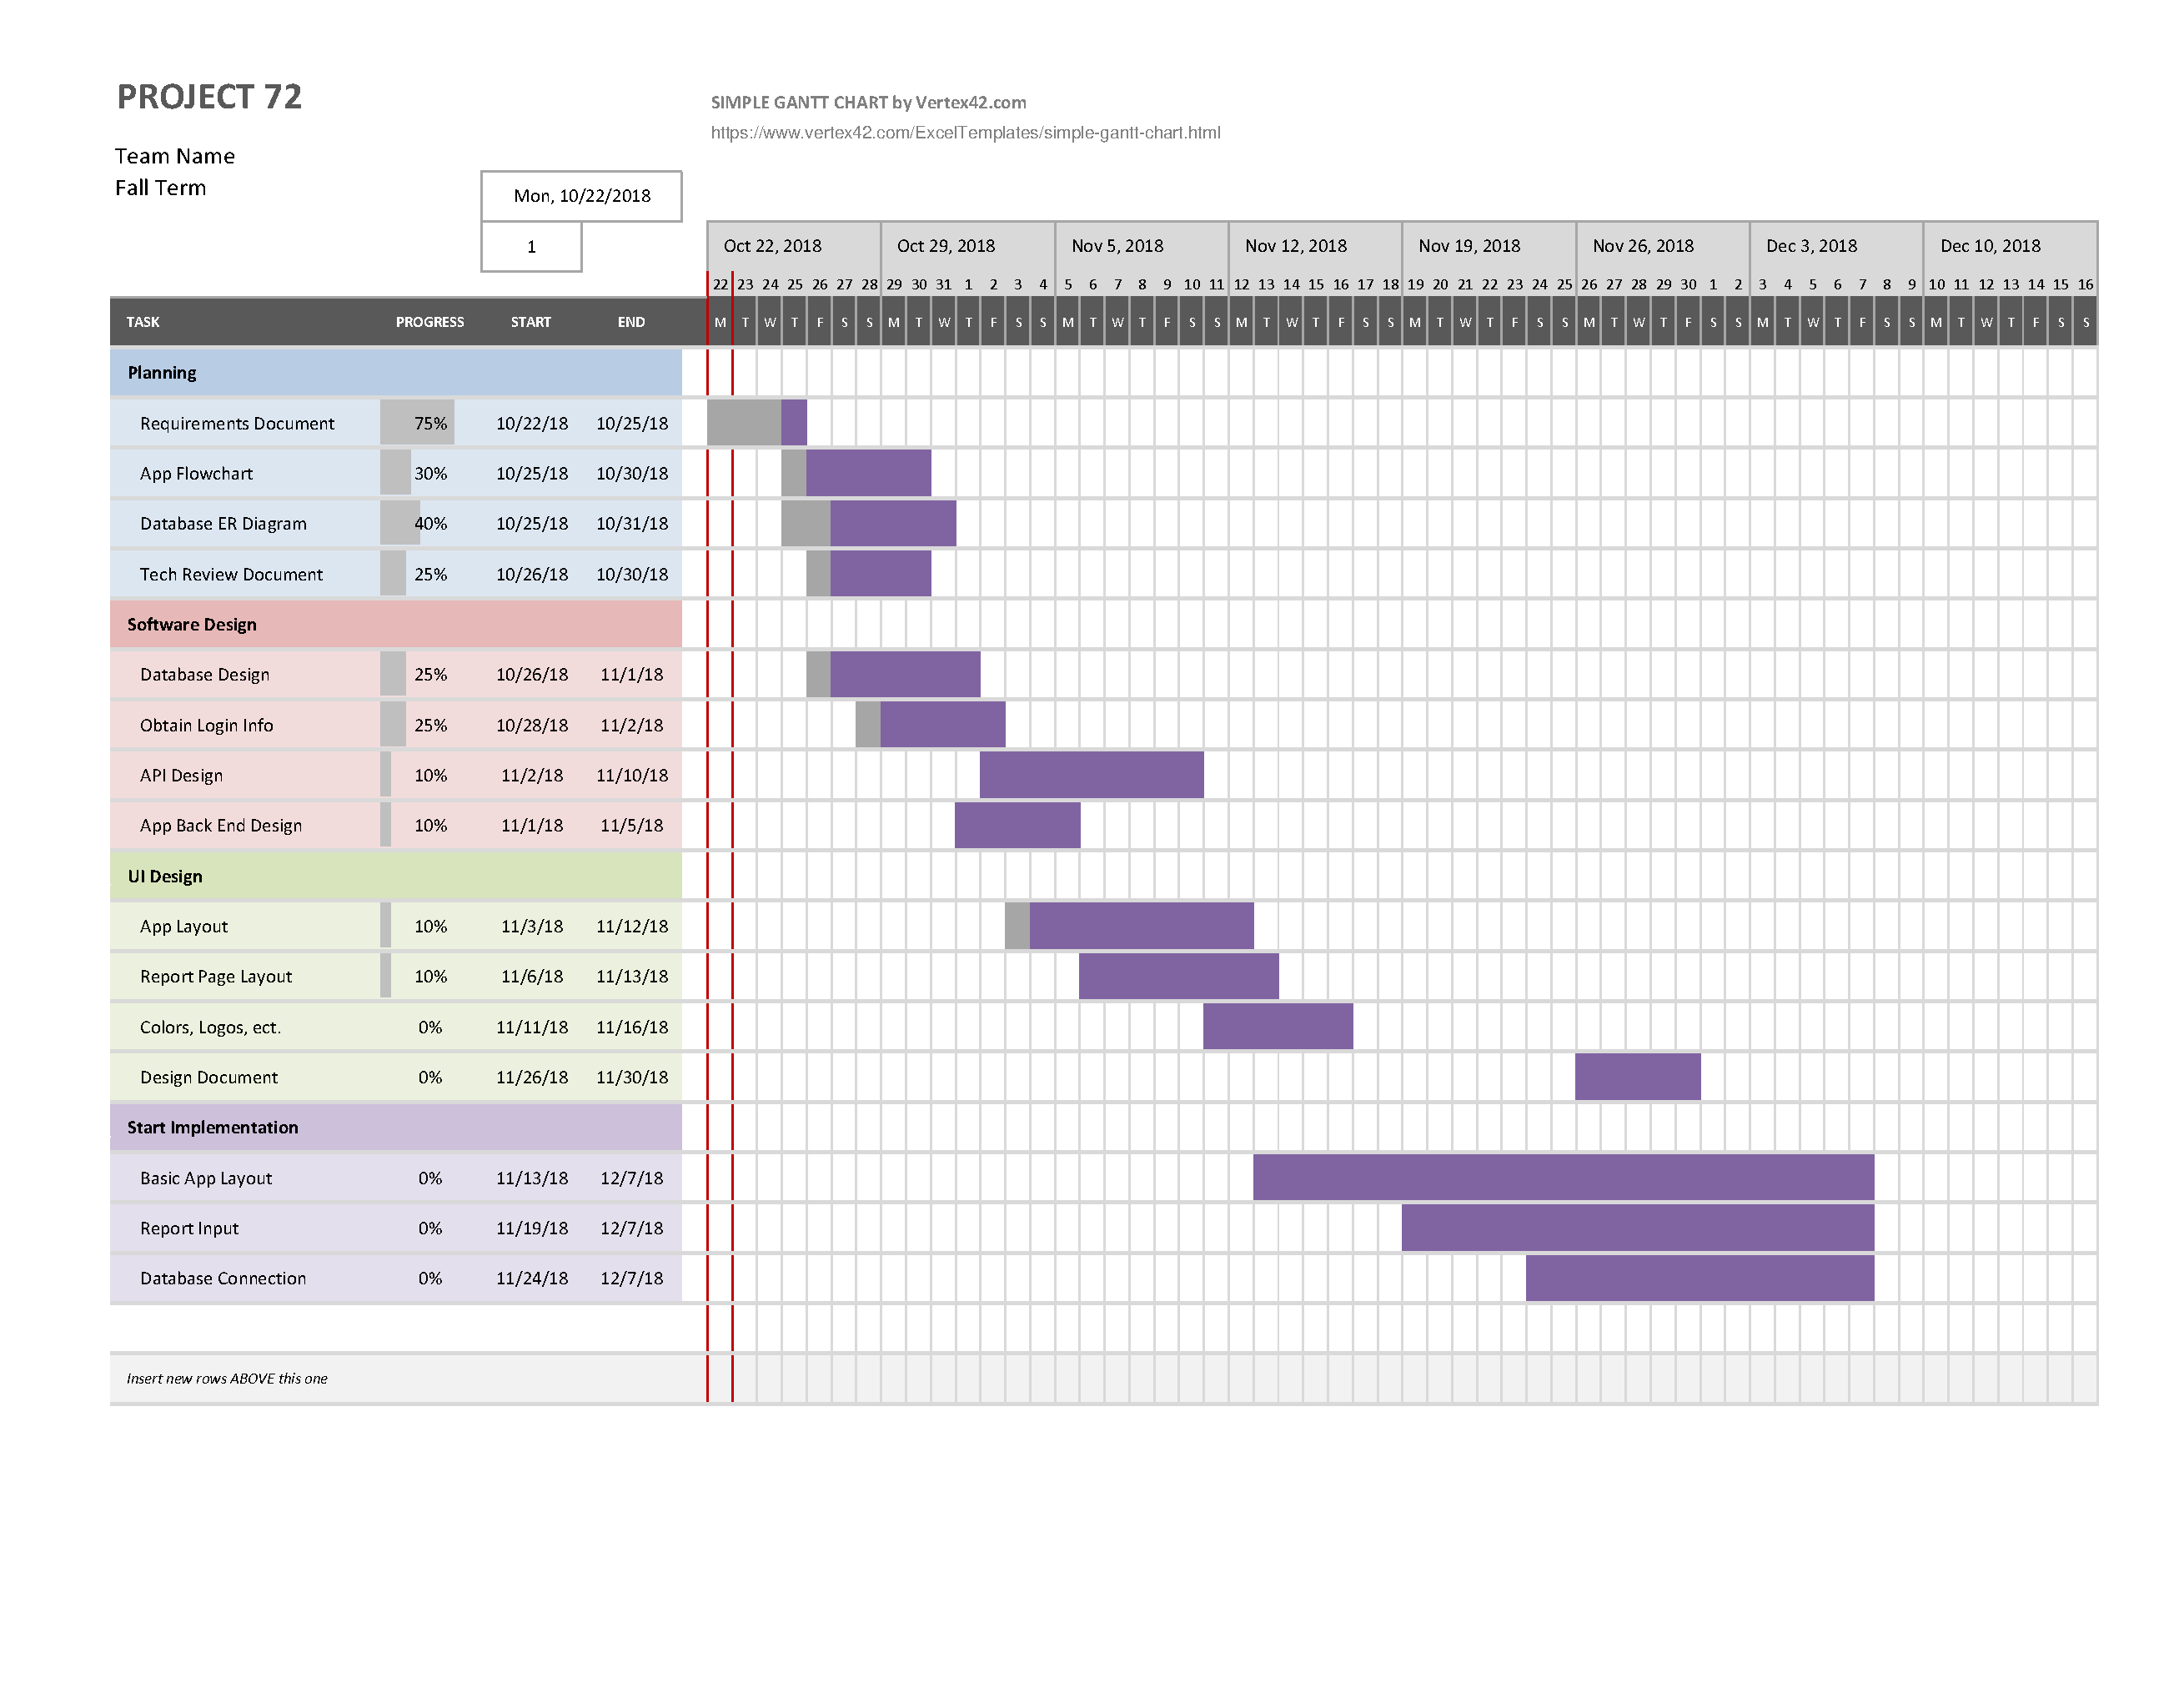
\includegraphics[scale=.45, angle=90]{GanttChart1.pdf}
}
\caption{Fall Term 2018}
\end{figure}

\begin{figure}[htp] \centering{
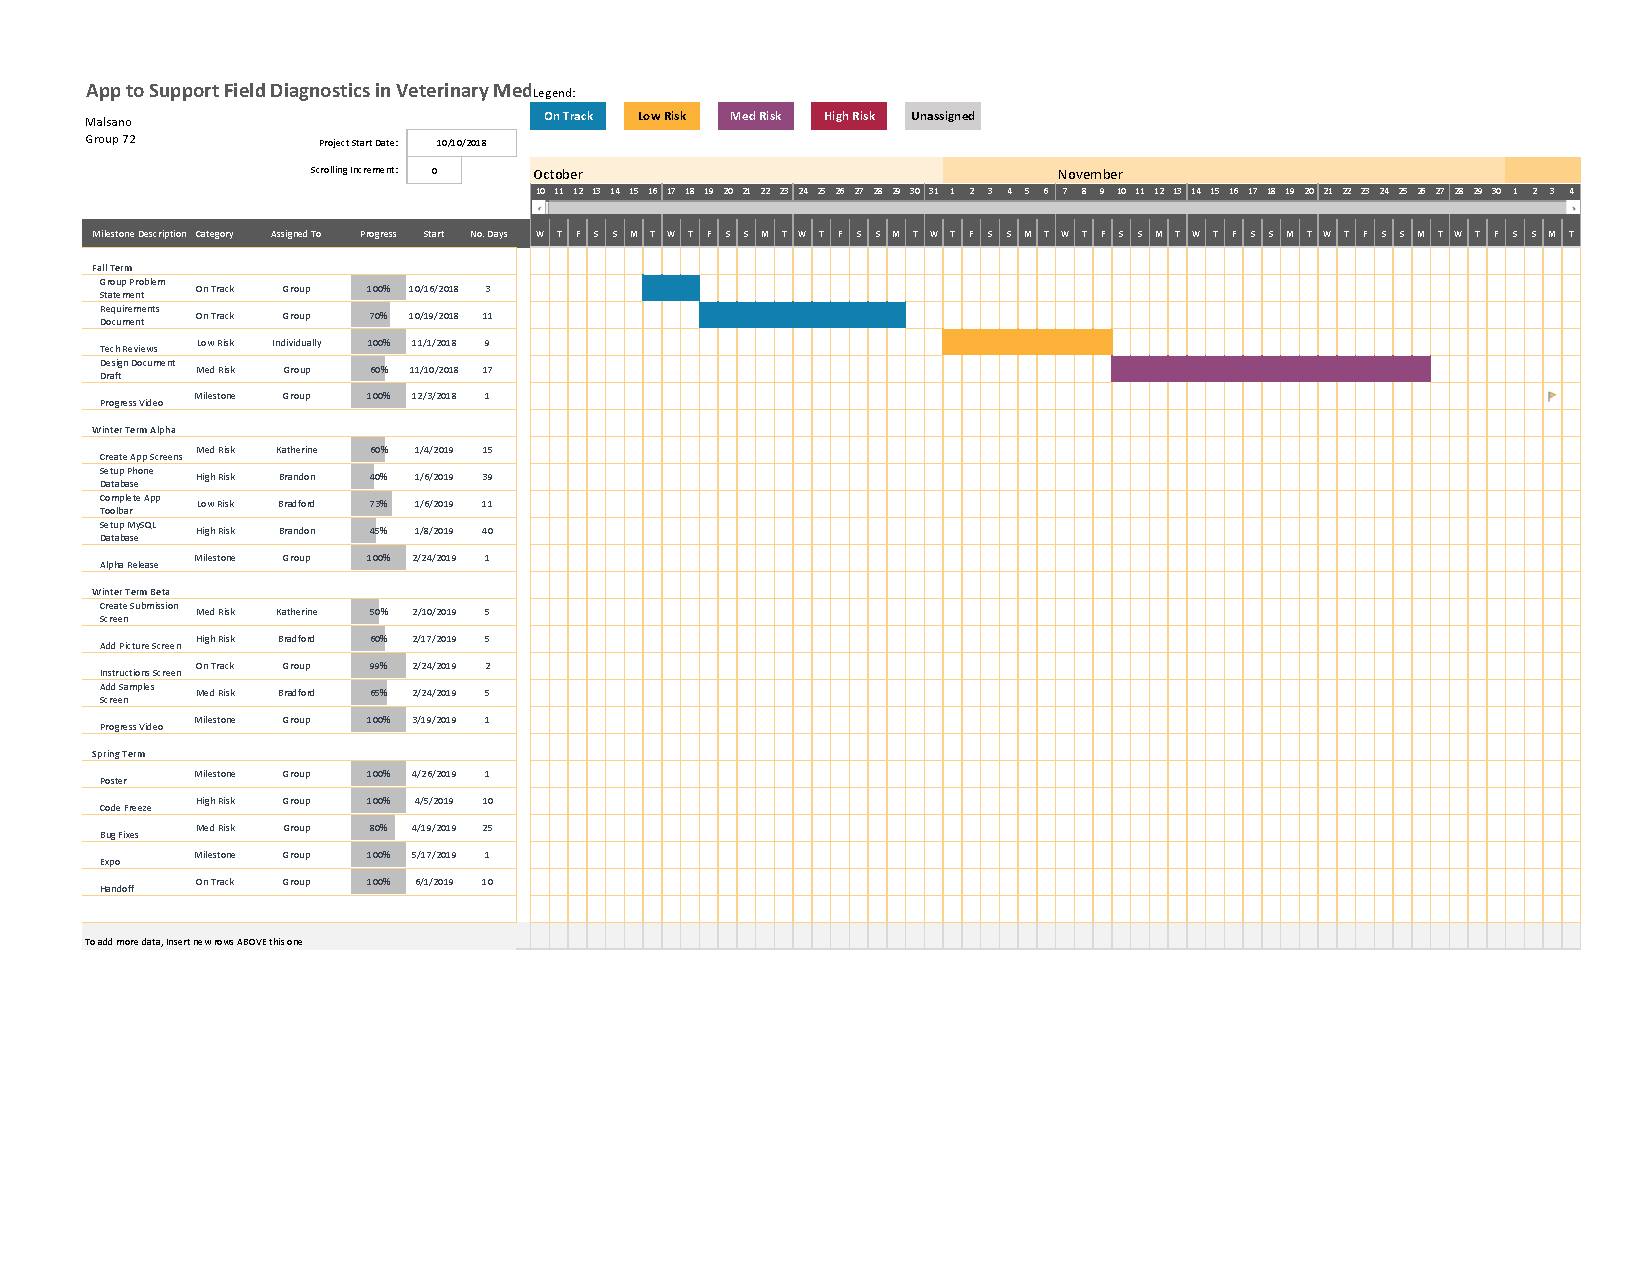
\includegraphics[scale=.8, angle=90]{FinalGantt1.pdf}
}
\caption{Final Gantt Chart Fall Term}
\end{figure}

\begin{figure}[htp] \centering{
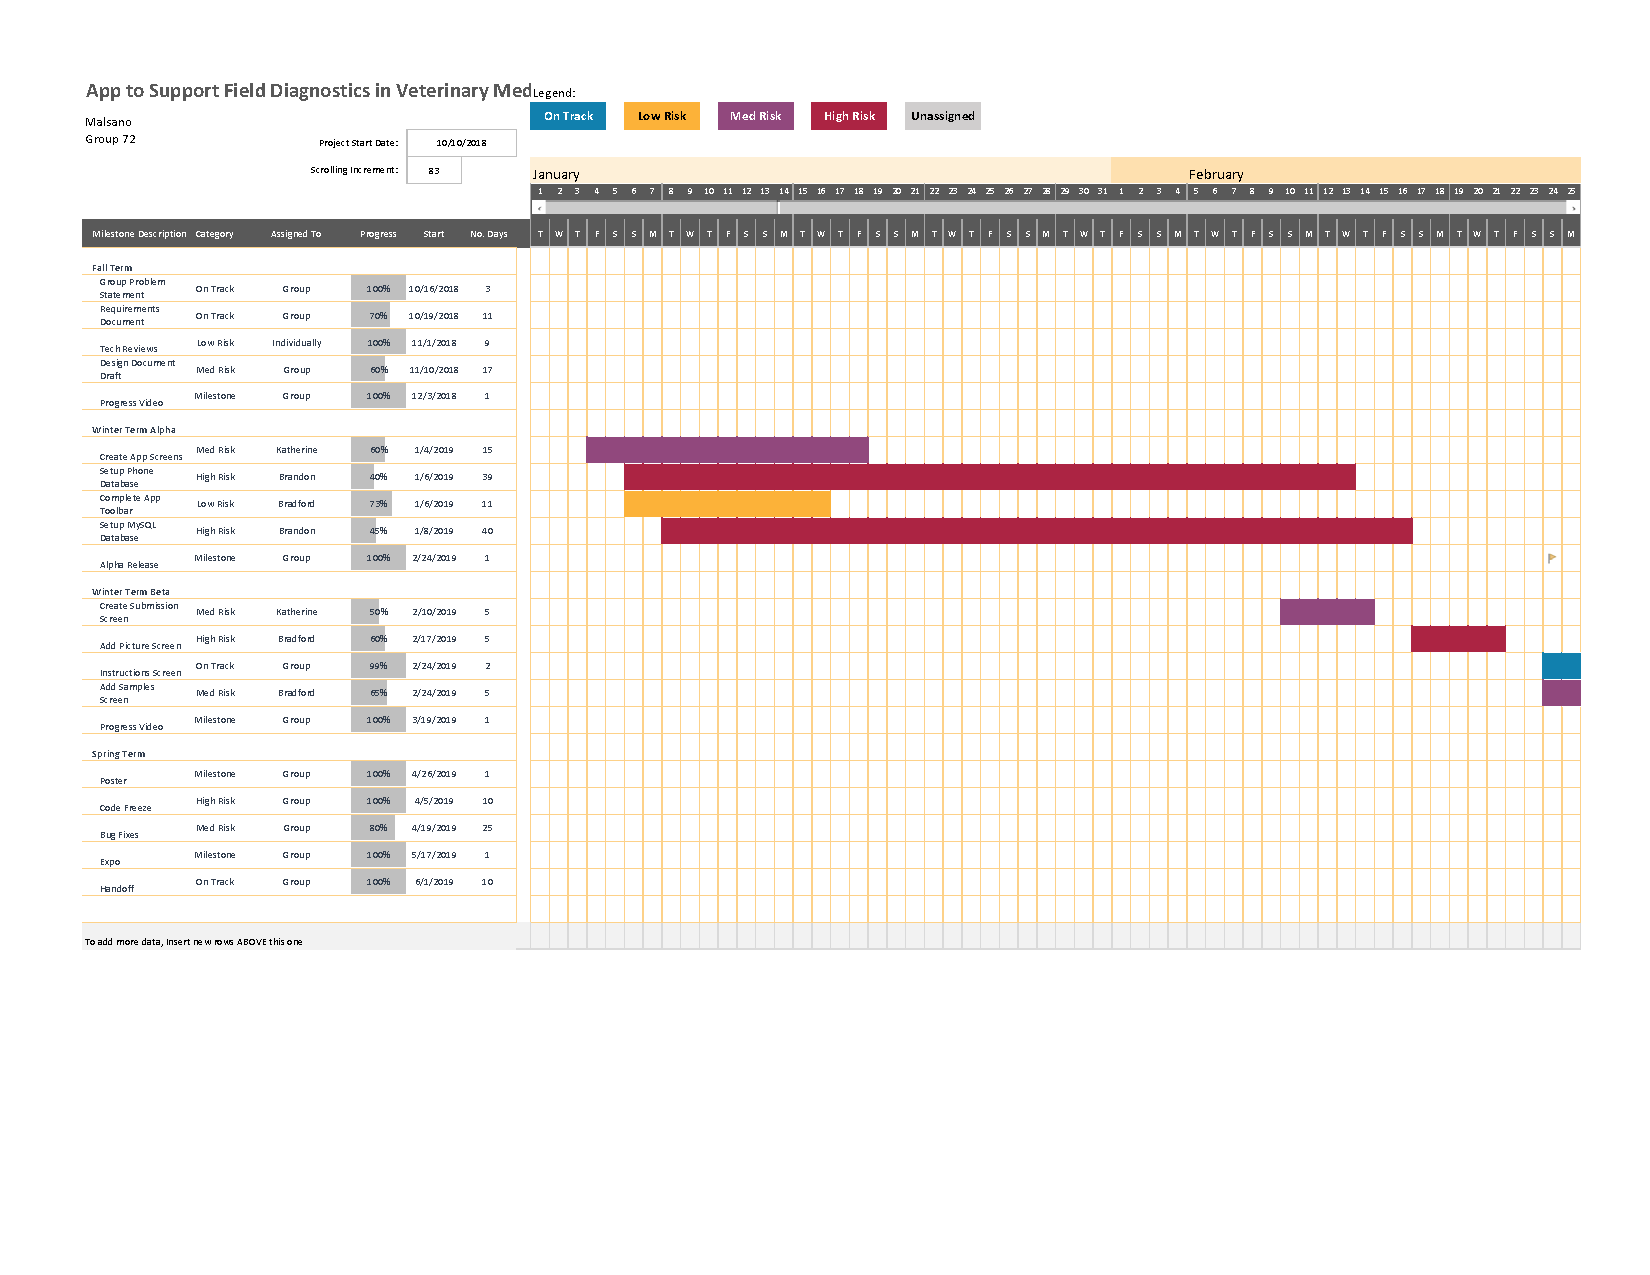
\includegraphics[scale=.8, angle=90]{FinalGantt2.pdf}
}
\caption{Final Gantt Chart Winter Term Alpha}
\end{figure}

\begin{figure}[htp] \centering{
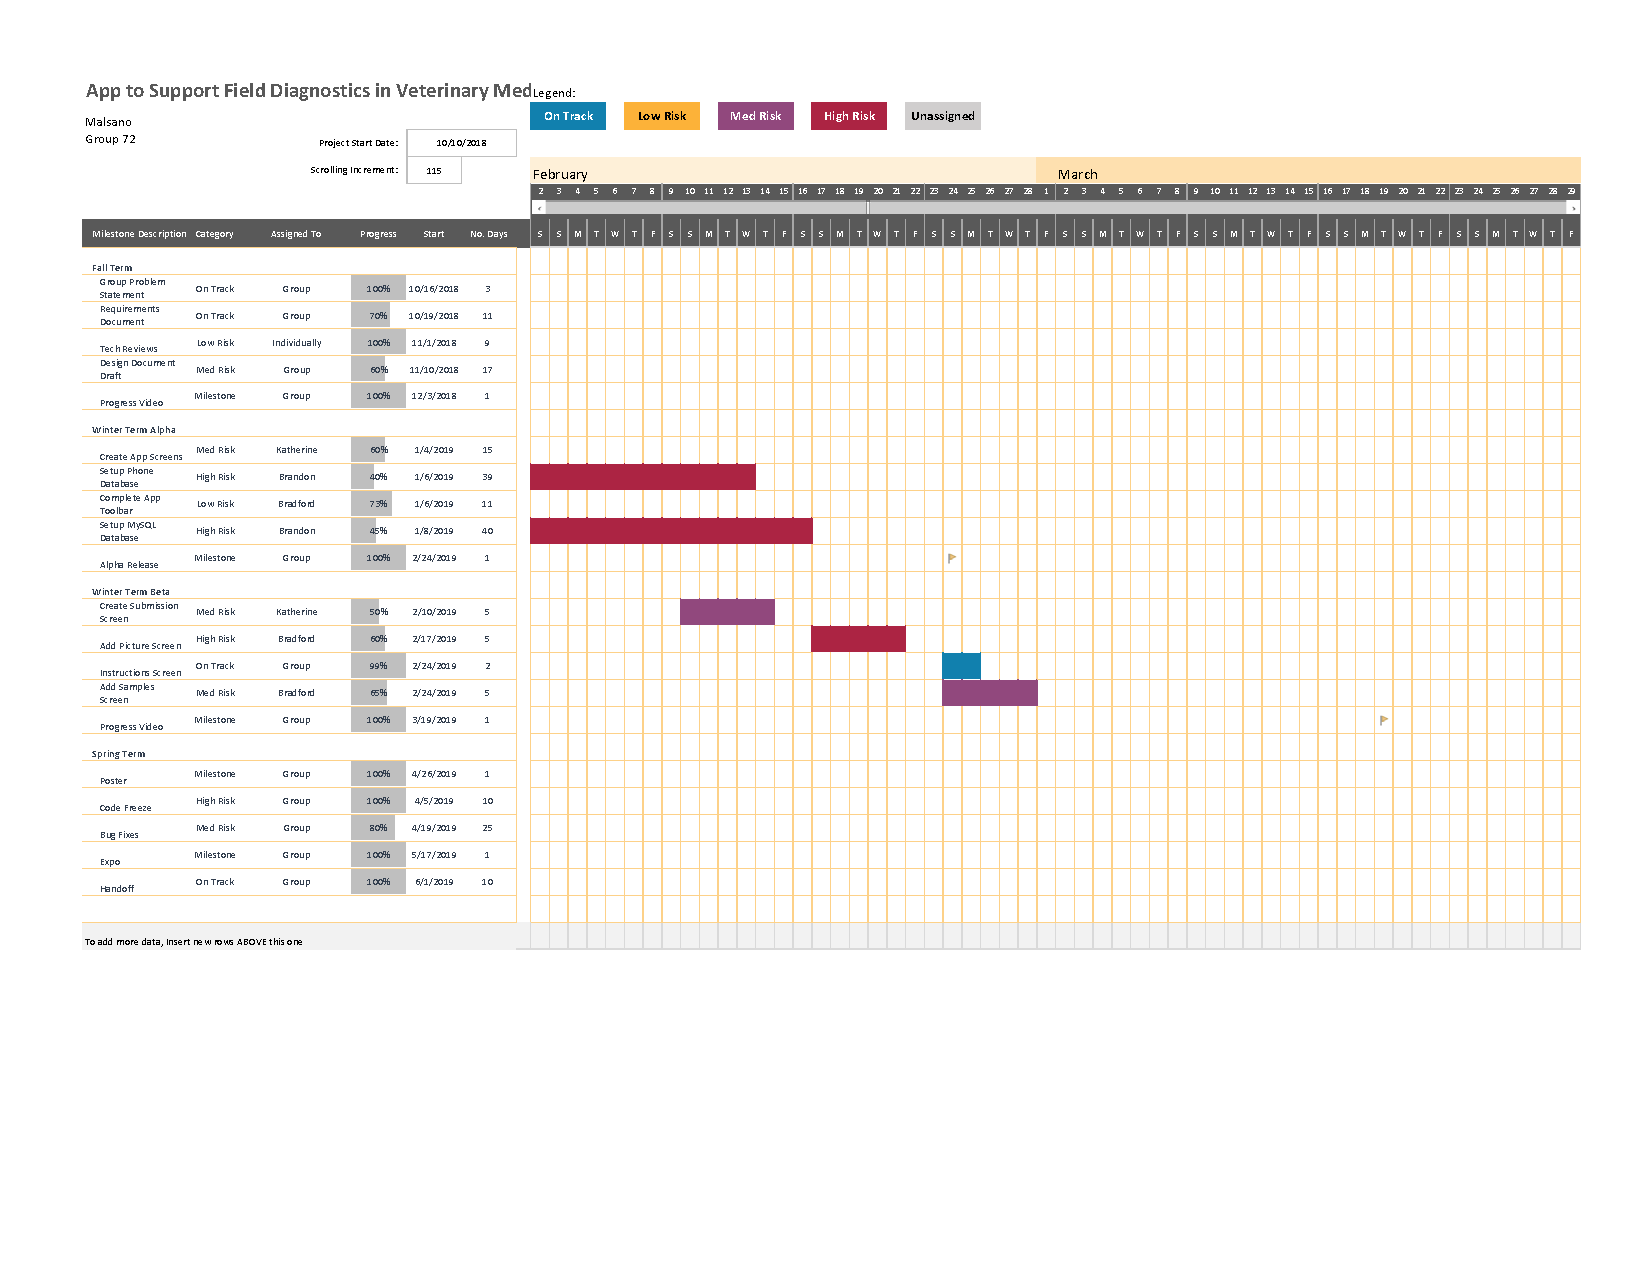
\includegraphics[scale=.8, angle=90]{FinalGantt3.pdf}
}
\caption{Final Gantt Chart Winter Term Beta}
\end{figure}

\begin{figure}[htp] \centering{
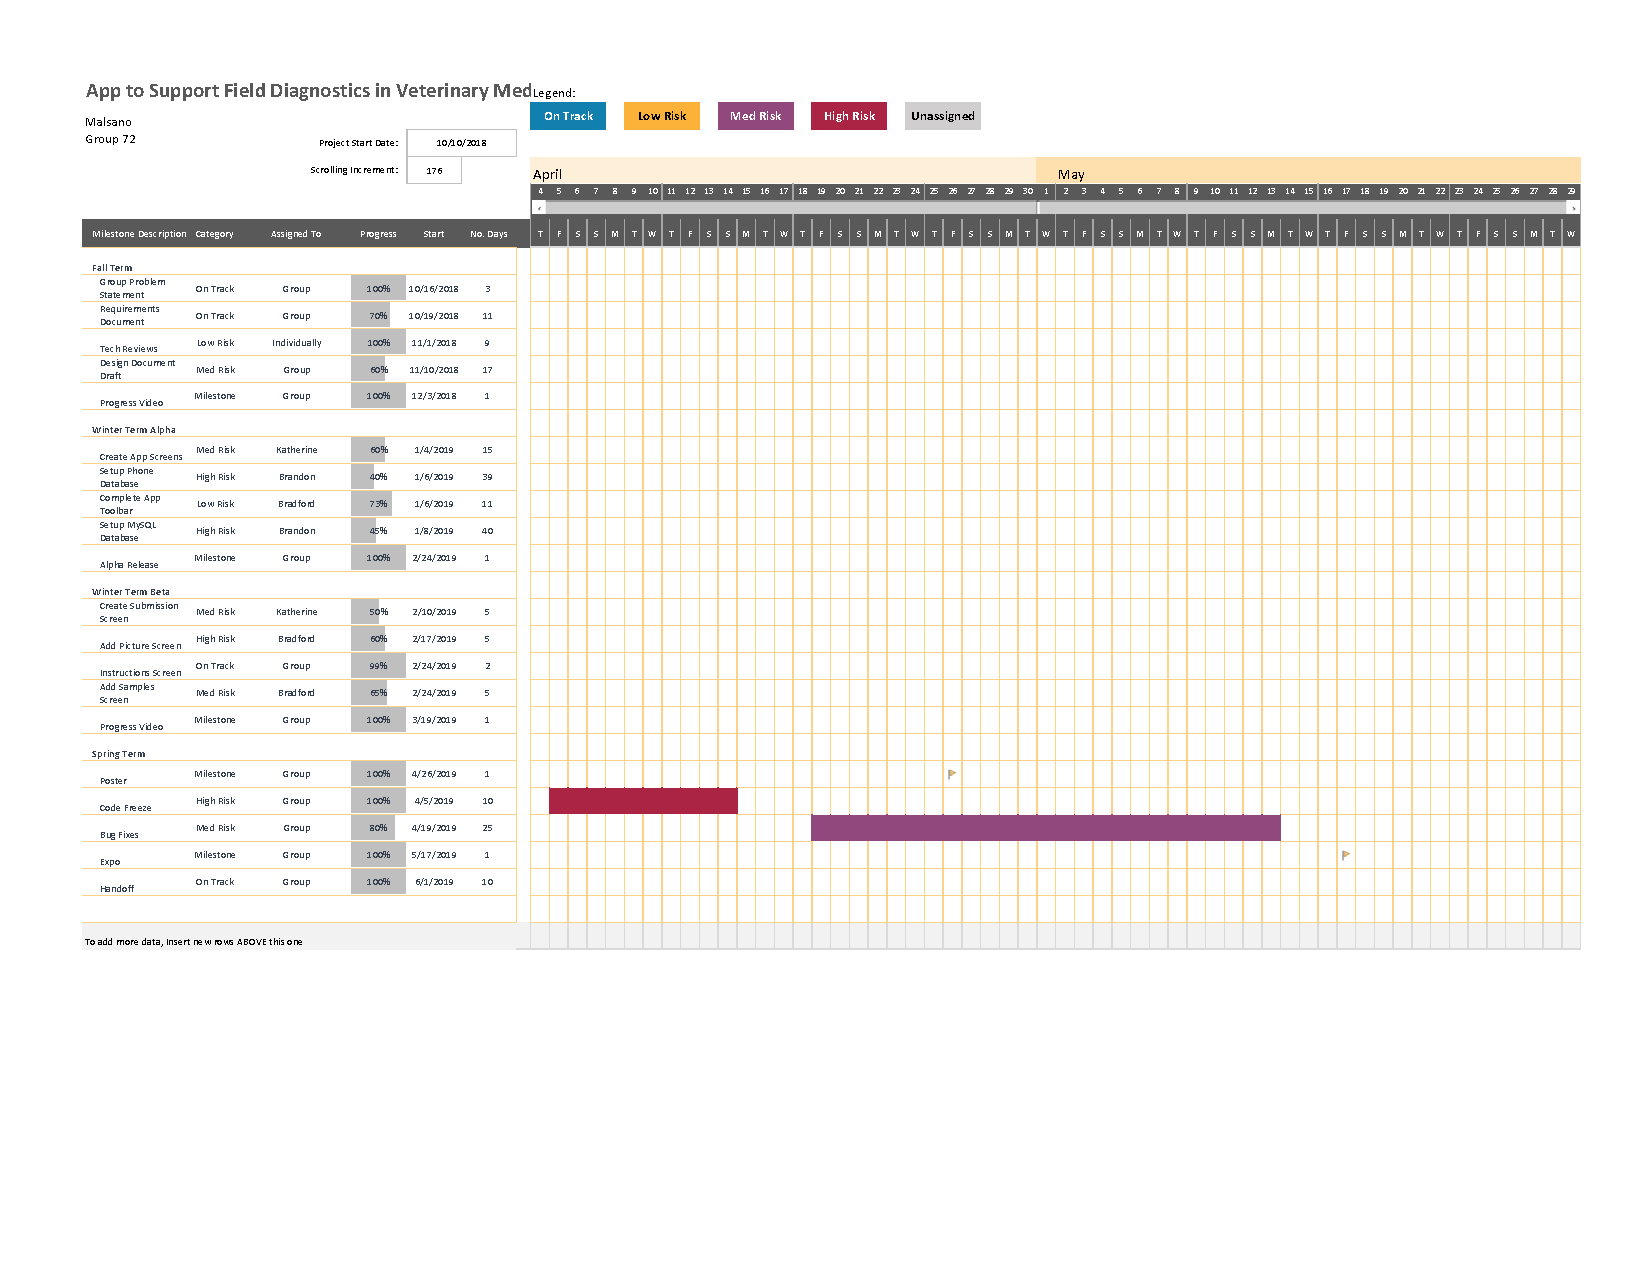
\includegraphics[scale=.8, angle=90]{FinalGantt4.pdf}
}
\caption{Final Gantt Chart Spring Term}
\end{figure}

 \section{Design Document}
 \subsection{Change Log}


\begin{table}[!hbt]
\begin{tabularx}{\textwidth}{|>{\setlength\hsize{.8\hsize}\setlength\linewidth{\hsize}}X|>{\setlength\hsize{1.1\hsize}\setlength\linewidth{\hsize}}X|>{\setlength\hsize{1.1\hsize}\setlength\linewidth{\hsize}}X|}
\hline

\hline
Section & Original & New \\
\hline
% col 1
Home Screen
&
% col 2
There will be four NavButtons
&
% col 3
\begin{itemize}
    \item Replaced "NavButtons" with "buttons"
\end{itemize}
\\

\hline
% col 1
Button
&
% col 2
3.2 NavButton
&
% col 3
\begin{itemize}
    \item Changed section item to "Buttons"
\end{itemize}\\

\hline
% col 1
Button
&
% col 2
This custom class will inherit from the Button class.
&
% col 3
\begin{itemize}
    \item Deleted text and explained that there will need to be onClick listeners.
\end{itemize}
 \\

\hline
% col 1
Button
&
% col 2
This class should also have getter and setter functions for each of the attributes.
&
% col 3
\begin{itemize}
    \item Replaced text with explanation that said the buttons will be added in the screen's layout XML file.
\end{itemize}
 \\

\hline
% col 1
Past Submissions Screen
&
% col 2
Each row will also have the Case ID in green text if it was successfully sent to the server.
&
% col 3
\begin{itemize}
    \item Changed it with explanation saying that each row will say when the submission was sent to the server.
    \item Added text saying that if the submission wasn't sent yet, then it will say "pending".
\end{itemize}
\\

\hline
% col 1
 View Submissions Screen
&
% col 2
The pictures of the submission will show up in a GridLayout. The pictures will initially just have a camera icon. Clicking on the icon will actually downloading the image.
&
% col 3
\begin{itemize}
    \item Deleted text and gave updated description of what information will be provided.
\end{itemize}
 \\

\hline
% col 1
Settings Screen
&
% col 2
There will be a login button that will prompt the user with a customized AlertDialog for their username and password to save their credentials to the phones local storage.
&
% col 3
\begin{itemize}
    \item Now says that clicking on a button will go to a different screen instead of having an AlertDialog.
\end{itemize}
 \\

\hline
% col 1
Add Samples Screen
&
% col 2
This section did not originally exist.
&
% col 3
\begin{itemize}
    \item Added description of the Samples Screen
\end{itemize} \\

\hline
% col 1
Create Submission Screen
&
% col 2
The icon will also have a badge, which will say the number of pictures that were added to the submission.
&
% col 3
\begin{itemize}
    \item Deleted part about badge.
    \item Added description about "Add Samples" button.
\end{itemize}
\\

\hline
% col 1
Create Submission Screen
&
% col 2
There will be a combination of text fields and dropdown menus.
&
% col 3
\begin{itemize}
    \item Added calendar fragments to the list
\end{itemize} \\

\hline


\end{tabularx}
\end{table}

\clearpage

% second table
\begin{table}
\begin{tabularx}{\textwidth}{|>{\setlength\hsize{.8\hsize}\setlength\linewidth{\hsize}}X|>{\setlength\hsize{1.1\hsize}\setlength\linewidth{\hsize}}X|>{\setlength\hsize{1.1\hsize}\setlength\linewidth{\hsize}}X|}
\hline
Section & Original & New \\
\hline

% col 1
App Pages
&
% col 2
 Each entry should be clickable and clicking on an entry will take the user to a detailed page of that submission, but  navigating to a submission's page won't be implemented in time for the Alpha.
&
% col 3
\begin{itemize}
    \item Removed part about the Alpha.
\end{itemize}
\\

\hline
% col 1
App Pages 
&
% col 2
 Submissions and Server Database - After creating a submission, the submission will automatically be sent to the server if there is a stable internet connection. If there isn't stable server connection, it will just be stored locally on the phone. Once there is an internet connection, the submissions will automatically be sent to the server.
&
% col 3
\begin{itemize}
    \item This item was removed.
\end{itemize}
\\

\hline
% col 1
Beta Level Release (Finals Week, Winter Term)
&
% col 2
At this point, a user will be able to create a submission and successfully send it to the server.
&
% col 3
\begin{itemize}
    \item Changed it so it says that submission is stored into the SQLite database instead of the server
\end{itemize}
\\

\hline
% col 1
Web Application
&
% col 2
\begin{itemize}
\item Users will be able to register a new account
\item Users will be able to login
\item Users will be able to see data on the database
\item Users will be able to see submissions that were created and sent to them
\item Users will be able to create comments on specific submissions
\end{itemize}  
&
% col 3
\begin{itemize}
    \item This section was removed.
\end{itemize}
\\
\hline

% col 1
Drafts
&
% col 2
When a user is creating a submission, they will have the option to save their current submission as a draft and won't necessarily submit it. There will be a button at the bottom of the "Create Submission" screen that says "Save Draft". Clicking on it will automatically save the draft and return the user to the home page. Additionally, the home page will have a button called "View Drafts", and clicking on this button will take the user to a page that shows all the user's saved drafts. The drafts will be listed in a table similar to what is shown in the "View Submissions" screen. Clicking on a draft will take the user to the "Create Submission" page where all of the information saved in the draft is automatically filled out for the user.
&
% col 3
\begin{itemize}
    \item This section was moved to the Beta Level Release Section (now section 6.1.3). 
\end{itemize}
\\
\hline

\end{tabularx}
\end{table}

\clearpage

% third table
\begin{table}
\begin{tabularx}{\textwidth}{|>{\setlength\hsize{.8\hsize}\setlength\linewidth{\hsize}}X|>{\setlength\hsize{1.1\hsize}\setlength\linewidth{\hsize}}X|>{\setlength\hsize{1.1\hsize}\setlength\linewidth{\hsize}}X|}
\hline
Section & Original & New \\

\hline
% col 1
Settings Page (6.3.5) 
&
% col 2
This page will have two options that the user can click on ("Manage account" and "Delete App").
\begin{itemize}
\item Manage Account - Clicking on this link will send the user to the website
\item Delete App - Deletes app 
\end{itemize}
&
% col 3
\begin{itemize}
    \item This was removed.
\end{itemize}
 \\

\hline
% col 1
Instructions Screen (6.3.6)
&
% col 2
This page will have four sections (Registering a New User, Creating a Submission, Sending a Submission, and App Usage) that have information underneath them detailing how to do each process
\begin{itemize}

\item Registering a New User - Provides a link to the web page that allows users to create an account
\item Creating a Submission - Details how to navigate to the page to create a report and how drafts work 
\item Sending a Submission - Explains that clicking on the "Submit" button at the bottom of a Submission will send it to the server if there is an internet connection. If there isn't an internet connection, then it will automatically send when the user regains a connection 
\item App Instructions - Provides a broad explanation on how to use the application
\end{itemize}
&
% col 3
\begin{itemize}
    \item This section was moved to the Beta Level Release section of the timeline.
\end{itemize}
 \\
\hline

% col 1
App Pages
&
% col 2
The toolbar will have white text and a background color that depends on what page the user is in (blue for "Create Report", red for "View Past Reports", and green for "View Drafts").
&
% col 3
\begin{itemize}
    \item Deleted part about the background color.
\end{itemize}
 \\

\hline


\end{tabularx}
\end{table}

\clearpage
% fourth table
\begin{table}
\begin{tabularx}{\textwidth}{|>{\setlength\hsize{.8\hsize}\setlength\linewidth{\hsize}}X|>{\setlength\hsize{1.1\hsize}\setlength\linewidth{\hsize}}X|>{\setlength\hsize{1.1\hsize}\setlength\linewidth{\hsize}}X|}
\hline
Section & Original & New \\
\hline
% col 1
App Pages
&
% col 2
On all pages but the home screen, there will be back arrow on the left of the header bar.
&
% col 3
\begin{itemize}
    \item Added "Add Pictures" screen and "Add Samples" screen to list.
    \item Added description about back arrow
\end{itemize}
 \\
\hline

% col 1
6.2.2 Create Submission Screen
&
% col 2
All of the missing fields will be added. The following information will be collected on this screen: 

\begin{itemize}
\item Group Name - Input using text field
\item Is this research? - Input using checkbox
\item VDL Account number - Input using number field
\item Has the user's information changed - Input using checkbox
\item Submitter's information

\begin{itemize}
\item Submitter 
\item Address - Input using text field
\item City - Input using text field
\item State - Input using text field
\item Zip - Input using text field
\item Phone - Input using text field
\item Fax - Input using text field
\item Email - Input using text field
\item Submitting Veterinarian - Input using text field
\end{itemize}


\item The Owner's information (if other than submitter)
\begin{itemize}
\item Owner 
\item Address - Input using text field
\item City - Input using text field
\item State - Input using text field
\item Zip - Input using text field
\item Phone - Input using text field
\item Previous Accessions - Input using text field
\item Copy Results To - Input using text field
\item Email/Fax 
\end{itemize}

\end{itemize}
&
% col 3
\begin{itemize}
    \item All of this was removed.
\end{itemize}
\\
\hline

\end{tabularx}
\end{table}

% fifth table
\clearpage
\begin{table}
\begin{tabularx}{\textwidth}{|>{\setlength\hsize{.5\hsize}\setlength\linewidth{\hsize}}X|>{\setlength\hsize{1.7\hsize}\setlength\linewidth{\hsize}}X|>{\setlength\hsize{.8\hsize}\setlength\linewidth{\hsize}}X|}
\hline
Section & Original & New \\
\hline

% col 1
6.2.2 Create Submission Screen
&
% col 2


\begin{itemize}


% here
\item Animal Identification
    \begin{itemize}
    \item Number - Automatically provided by app
    \item Name/identifier No. - Input using text field
    \item Species - Input using text field
    \item Breed - Input using text field
    \item Sex - Input using text field
    \item Date of Birth - Input using text/date field
	\item Date Specimens taken - Input using text field
    \item Date Specimens Submitted - Input using text field
    
    \item Number of each sample type
    
      \begin{itemize}
      \item Whole Animal - Input using number field
      \item Fresh Tissue - Input using number field
      \item Formalin Fixed Tissue - Input using number field
      \item Blood, whole - Input using number field
      \item Serum - Input using number field
      \item Plasma - Input using number field
      \item Milk - Input using number field
      \item Urine - Input using number field
      \item Voided - Input using checkbox
      \item Catherized - Input using checkbox
      \item Cystocentesis - Input using checkbox
      \item Fluid (and origin information) - Input using number field for sample number and text field for origin information
      \item Swab (and origin information) - Input using number field for sample number and text field for origin information
      \item Other (and origin information) - Input using number field for sample number and text field for origin information
      \end{itemize}
      
    \item Histopathology on Biopsy (and source information) - Input using checkbox and text field for source information
    \item Necropsy only - Input using checkbox
    \item Necropsy with Histology - Input using checkbox
    \item Necropsy and Complete Diagnostic Work up - Input using checkbox
    \item Other - Input using checkbox and textfield 
    \end{itemize}
    
\item Care of Remains (Small animals only)

\begin{itemize}
\item Routine Disposal - Input using checkbox
\item Cremation (Specify Company) - Input using checkbox
\end{itemize}

\item A clickable button that navigates the user to a screen that will allow them to input pictures. The details of this page will be outlined in a later section.

\item A clickable button that says "Save Draft".

\item A clickable button that says "Submit". Clicking on this button will finish the submission and save its details to the phone's local database.
\end{itemize}
&
% col 3
\begin{itemize}
    \item Replaced this with an updated list of what is being collected and how the data is being collected.
    \item Added description about "Add Pictures", "Save Draft', "Add Samples", and "Submit" buttion.
\end{itemize}
\\
\hline

\end{tabularx}
\end{table}

\clearpage

% Sixth table
\begin{table}
\begin{tabularx}{\textwidth}{|>{\setlength\hsize{.8\hsize}\setlength\linewidth{\hsize}}X|>{\setlength\hsize{1.1\hsize}\setlength\linewidth{\hsize}}X|>{\setlength\hsize{1.1\hsize}\setlength\linewidth{\hsize}}X|}
\hline
Section & Original & New \\
\hline
% col 1
6.2.9 Add Samples Screen
&
% col 2
This section didn't exist before.
&
% col 3
\begin{itemize}
    \item Added description about the screen and how data is being collected.
\end{itemize}
\\
 \hline %database changes
 Database & Table SickElement & Now called Patient\\ 
 \hline
 Database & Column in Table SickElement called SickElementName & Now Called PatientName\\
 \hline
 Database & Replies For submission table will connect Submission and Replies & This table has been dropped and the columns from the table are moved to replies\\
 \hline
 Database & Client table will hold the information for clients, Pathologist table will hold information pertaining to a Pathalogist  & These tables have been dropped and the columns have been moved to the user table\\
\hline Database & There was none previously & Added column Submission Review to the Report Table. This column will hold the initial review a Pathologist has regarding a submission.\\
\hline Database & There was none previously & Added the Date Closed Column to the Report table. This column will hold the data of when a report has been closed\\
\hline Database & The tables will have the naming convention of ALL CAPS & The tables have now been changed to have the naming convention of Camel Case\\
\hline Database & The tables primary keys will have the naming convention of camel case & The Primary keys will now have the naming convention primary\_ID\\
\hline Database & The Image table 
& 
\begin{itemize}
    \item This has been renamed as the Picture Table
    \item The column imagePath has been renamed picturePath
    \item The column image\_ID has been renamed Picture\_ID
\end{itemize} 
\\
\hline Database & The User table will have a column called Authorized & The column has been renamed Authenticate. \\
\hline Database & The table submission table will have a primary key of internal\_id & It has now been changed to master\_Id and the foreign keys have reflected that.\\ 
\hline
Glossary & There was non previously. & Added, "Reply - A message sent between the user and the client" to the glossary.\\
\hline
% col 1
Settings
&
% col 2
The settings screen will have a logout button that will remove the users account credentials from the phone’s local storage. They will need to authenticate their account again before they can save or send a submission.
&
% col 3
Clarified that users only have to log-in whenever they send data to the server. They can save data locally without having to authenticate.
 \\
\hline

% col 1
Connection between Databases
&
% col 2
Once the new ID is given to the submission and all of the connections to the submission are updated,
then the submission will be added to the MySQL database. This process is done by turning the submission and it’s
components would then be used by an API to connect to the database to upload the information into storage.
&
% col 3
\begin{itemize}
    \item Replaced "new ID" with "master\_ID".
    \item Reworded last sentence
\end{itemize}
 \\
\hline
\end{tabularx}
\end{table}

\subsection{Introduction}
The completed project components are intended to serve as a means of communication between personnel in the field and pathologists in the laboratory. It's purpose is to improve a team's ability to perform remote diagnostics by providing a convenient way for teams to communicate information. The OVDL wants a native Android mobile application that collects field data and images, stores the information on a native SQLite database, sends them to the lab's MySQL database, and gets real time feedback from the lab. The lab will interact with the database and user's submissions through the website. 

\subsection{Android Application}
\subsubsection{Home Screen}
There will be four buttons (described later). Clicking on each button will take the user to the corresponding page. The NavButtons will be contained in a vertical linear layout. Here is a list of each button and what their attributes will be:
\begin{itemize}
\item A button with an image of a person’s shape for the image, light green for the background color, and “"Create Account"” for the text. Clicking on this button will open up the web browser and take the user to the registration page
\item A button with a plus icon for the image, blue for the background color, and "“Create submission”" for the text
\item A button with a closed folder icon for the image, red for the background color, and “"View submission"” for the text
\item A button with an icon an open folder for the image, dark green for the background color, and “"View Drafts”" for the text
\end{itemize}

\begin{center}
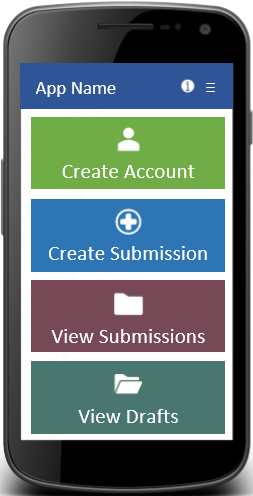
\includegraphics[height=8cm]{homescreen.png}
\end{center}
\captionof{figure}{Home Screen Mockup}


\subsubsection{Buttons}
These buttons must have onClick listeners that will take the user to the appropriate page once clicked. Their attributes should include an image, background color, and text. All the text color will be set by default to white. These buttons will be added in the screen's layout XML file.

\subsubsection{Toolbar Menu}
This will use the Toolbar class. Every page will have a toolbar, and the text in the toolbar will be the same as the current screen's name. There will be an overflow menu on the right of the toolbar with the following options: "Home", "Create submission", "View Submissions", "Instructions", and "Settings". Clicking on one option will take the user to the corresponding page. 
\newline
\begin{center}
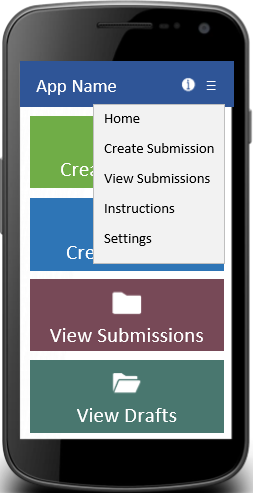
\includegraphics[height=8cm]{menuscreen.png}
\end{center}
\captionof{figure}{Menu Screen Mockup}

\subsubsection{Create Submission Screen}
There will be a combination of text fields and dropdown menus. The Spinner class will be used for the drop down menus and the EditText class will be used for text fields. There will be a button that says "Submit". Clicking on this button will create a submission in the phone's database and save all the submitted information. It will then try to send the submission to the database if there is an internet connection. There will also be a button that says "Save Draft", which will store the current draft with all its filled out information on the phone's database. There will also be a button with a camera icon on it. Clicking on it will take the user to the page where they can add and remove pictures to the submission. The icon will also have a badge, which will say the number of pictures that were added to the submission.
\newline
\begin{center}
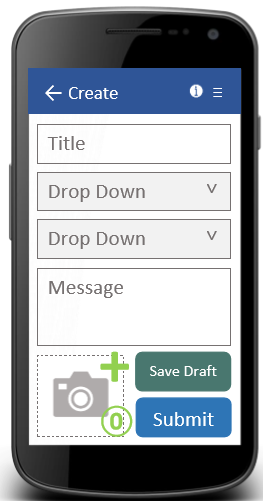
\includegraphics[height=8cm]{createscreen.png}
\end{center}
\captionof{figure}{Create Screen Mockup}

\subsubsection{Adding Pictures Screen}
This screen will use a grid layout. Each element will be of the ImageButton class. If a picture hasn't been added to a cell, then the cell's image will be a camera icon. If a picture has already been added, then the image will be the actual picture that was added. There will also be a floating, circular button on the bottom right of the screen with a checkmark icon. It will be of the FloatingActionButton class. Clicking on it will save the images and return the user back to the "Create" screen. The grid will have the following properties:
\newline
\begin{center}
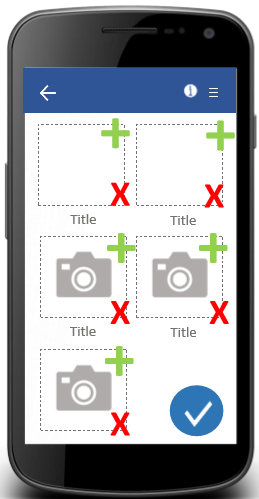
\includegraphics[height=8cm]{picturesscreen.png}
\end{center}
\captionof{figure}{Picture Screen Mockup}

\begin{itemize}
\item The grid will have two total columns
\item The first column will have three elements
\item The second column will have two elements
\end{itemize}

\subsubsection{Past Submissions Screen}
This screen will have a ListView with a Custom Adapter in order to populate the rows. Each row will have the title of the submission and the date it was created. Each row will say when the submission was sent to the server. If the submission hasn't been sent yet, then it will say "pending". Clicking on an entry will navigate the user to the detailed page of that submission.

\subsubsection{View Submissions Screen}
This screen will have a vertical LinearLayout where all of the information in the submission is added to the layout. This screen will show all content relevant to the submission such as the title, comment, samples, patient information, pictures, and replies.
\newline
\begin{center}
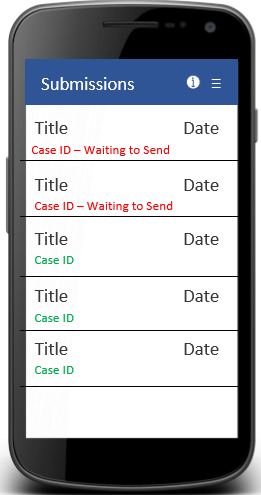
\includegraphics[height=8cm]{submissionscreen.png}
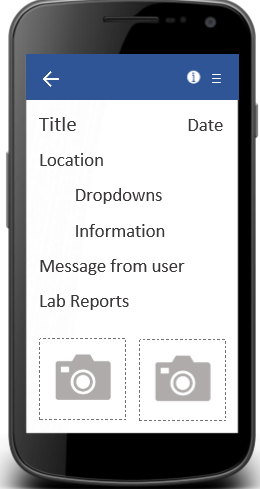
\includegraphics[height=8cm]{detailsscreen.png}
\end{center}
\captionof{figure}{Submissions and Details Screen Mockups}

%Katherine's Components
\subsubsection{Settings Screen}
The settings screen will have a logout button that will remove the users account credentials from the phone’s local storage. They will need to authenticate their account again before they can send a submission. There will be a login button that the user can click on to go to a different screen and input their login credentials. These credentials will be saved to the phone's local storage. To do this they must have an internet connection so their credentials can be matched in the database. 
\begin{center}
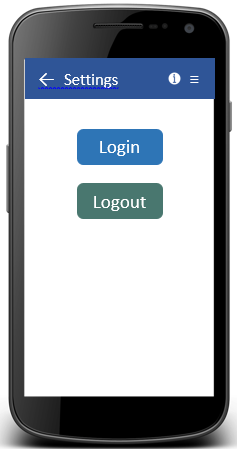
\includegraphics[height=8cm]{settingsscreen.png}
\end{center}
\captionof{figure}{Settings Screen Mockup}

\subsubsection{Instructions Screen}
The instructions screen will have lists of steps explaining how to use the app, how to register an account, how to create a submission, and how to send messages attached to the submissions. There will also be a link to the website and contact information for the OVDL. 
\newline
\begin{center}
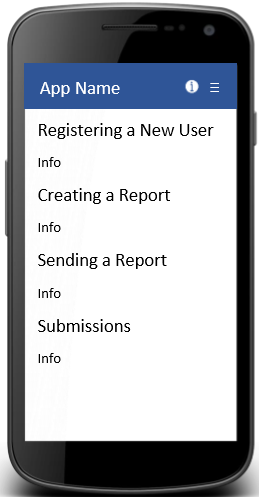
\includegraphics[height=8cm]{instructionsscreen.png}
\end{center}
\captionof{figure}{Instructions Screen Mockup}

\subsection{Database}
\subsubsection{Overview}
This project will utilize two databases using the structure presented in the figure below. One database is a MySQL database which will be storing the majority of the information for the app. This will be stored on an apache server and the information will be accessed using a web interface. Our second database is SQLite. The reason for this second database is to allow field workers to store information on the app while not connected to the internet. Instead the database will be stored locally within the phone and will only contain the current user's information.

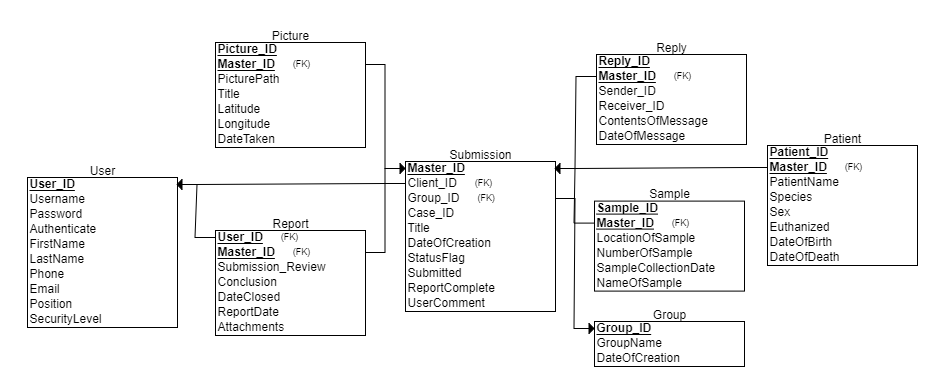
\includegraphics[height = 8cm]{ER_diagram.png}
\captionof{figure}{ER Diagram 4/14/19}

\subsubsection{Data Dictionary}
\begin{itemize}
\item User:\newline
The User table will contain all the information for a user in our database. This includes their UserName, password, and their contact information. This table will also include the Position if they have one and if their securityLevel 
\begin{itemize}
\item User\_ID: The primary key which is a unique integer value generated using a running total. Created when a new user is added to the table.
\item Username: A unique varchar(16) value created when a user creates an account using the web interface.
\item Password: A varchar(16) value created when a user creates an account using the web interface.
\item First Name: A varchar(30) value containing the user's first name.
\item Last Name: A varchar(30) value containing the user's last name.
\item Phone Number: A varchar(16) value containing the user's phone number in "XXX-XXX-XXXX" format.
\item Email: A varchar(40) value containing the user's email address.
\item Authorized: A binary value representing if a user has permission to modify reports, delete reports, etc.
\item Position: A varchar(60) value containing what position a user holds. (Assistant, Director, etc.)
\item Security Level: An interger value used to determine what permissions a user is able to use.
\end{itemize}

\item Submission:\newline
The submission table contains submissions a Client creates and then sends to a Pathologist to review.
\begin{itemize}
\item Master\_ID: The primary key for the Submission table. It is created using a running total on the SQLite database.
\item Client\_ID: A foreign key from the Client table to determining which client has created the report.
\item Case\_ID: An integer number created by using the last two digits of the year and then a six digit running total. It's primary use is to allow a pathologist to easily recognizing what submission they are working on. May be dropped in the future when the Use of this app expands. 
\item Group\_ID: A foreign key from the Group table which holds what group this submission is apart of. Defaulted to blank.
\item Title: A varchar(255) value containing the title a Client Created. The title has to be unique for the client only.
\item DateOfCreation: A datetime value representing the date the submission was first created. Formated as "YYYY/MM/DD HH:MM".
\item StatusFlag: An integer value represented the stage of a submission. 0, for draft, 1 for submitted, 2 for review, 3 for closed.
\item Submitted: A datetime value representing when the submission was sent to the MySQL database. Formated as "YYYY/MM/DD HH:MM".
\item ReportComplete: A datetime value for when the submission has been closed and the reports for the submission have been finished. Formated as "YYYY/MM/DD HH:MM".
\item UserComment: A varchar(255) value containing the comments a Client inputed when they where creating the submission.
\end{itemize}

\item Picture:\newline
The Picture table contains the images used in a submission. There could be many images which belong to the same submission. Also contains where the image was taken, when it was taken, and a Client created title.
\begin{itemize}
\item Picture\_ID: The primary key for the image table. Created using a running total for the specific submission.
\item Master\_ID: A foreign key from the Submission table and a primary key in combination with Image ID.
\item PicturePath: A varchar(255) containing the image file.
\item Title: A varchar(255) containing a user created title. Only has to be unique to the submission. 
\item Latitude: A floating point value containing the latitude coordinates.
\item Longitude: A floating ponit value containing the longitude coordinates.
\item Date Taken: A datetime value containing when the picture was taken. Formated as "YYYY/MM/DD HH:MM".
\end{itemize}

\item Patient:\newline
The Patient table contains the information regarding the animal in a submission. Such as the animal's name, it's sex, etc.
\begin{itemize}
\item patient\_ID: A primary key, an integer value which is generated with a running total on the SQLite database.
\item Internal ID: A foreign key from the submission table. A primary key in combination with the patient\_ID.
\item patient\_Name: A varchar(30) value contain a Client created name for the animal.
\item Species: A varchar(30) value containing what species the animal is.
\item Sex: A varchar(1) value containing the sex of the animal. M for male, and F, for female.
\item Euthanized: A binary value representing if the animal is euthanized or not.
\item DateOfBirth: A date value representing the birthday of the animal. Formated as "YYYY/MM/DD".
\item DateOfDeath: A date value representing the date of death for the animal. Formated as "YYYY/MM/DD".
\end{itemize}

\item Sample:\newline
The Sample table contains the information associated with the sample of the submission. 
\begin{itemize}
\item sample\_ID: A primary key in the form of an integer value. Generated with a running total on the SQLite Database.
\item master\_ID: A foreign key from the Submission table. Also a primary key in combination with Sample ID.
\item LocationOfSample: A varchar(255) value which contains the information of where the sample was taken from. For example Right leg, or blood from mouth.
\item NumberOfSample: An integer representing the amount of a sample taken.
\item SampleCollection Date: A date value representing when the sample was collected. Formated as "YYYY/MM/DD".
\item NameOfSample: A varchar(30) representing the name of the sample.
\end{itemize}

\item Group:\newline
The Group Table contains the information about a group. The name of the group and when it was created. A group must be created online before it can be used.
\begin{itemize}
\item group\_ID: The unique identifier for group. Incremented in the mysql Database
\item GroupName: a varchar(30) value which represent the group name. 
\item DateOfCreation: A date value representing when the group was created. Formated as "YYYY/MM/DD".
\end{itemize}

\item Reply:\newline
The Reply table stores information regarding the messages being sent back and forth between the Client and the Pathologist.
\begin{itemize}
\item reply\_ID: The primary key which is generated using a running total.
\item master\_ID: The second portion of the primary key. A foreign key to the Submission table
\item SenderID: The ID of who sent a reply.
\item ReceiverID: The ID of who received the reply.
\item ContentsOfMessage: A Varchar(255), which contains the actual message.
\item Date of Message: A date value for when the message was sent. Formatted as "YYYY/MM/DD HH:MM".
\end{itemize}

\item Report:\newline
The Report table is where the pathologist put the information from their review. Many Pathologist have the ability to review a submission but a report must pertain to a single submission.
\begin{itemize}
\item user\_ID: A foreign key from the Pathologist table and a primary key.
\item Master\_ID: A foreign key from the Submission Table and the other primary key for Report.
\item SubmissionReview: A varchar(255). The inital comments regarding a submission are placed here by a pathalogist in the mysql database through the use of an api.
\item Conclusion: A varchar(255). The last comments for a report. Stating the Submission is closed.
\item DateClosed: a date value which represents when the report was closed. Formated as, "YYYY/MM/DD"
\item ReportDate: A date value which represents when the report was created. Formated as "YYYY/MM/DD".
\item Attachments: A field for any attachments associated with the report.
\end{itemize}

\end{itemize}

\subsubsection{Connection between Databases}
When a submission is ready to be sent to the MySQL database a number of triggers activate. First the app will determine if the user is connected to the internet. If not the submission will not send and will be saved as a submission only locally on the phone(As a draft). If the user is connected to the internet, then a prompt will pop up asking the user to type in their username and password (If they have not done so already). Once they enter a correct username, a number will be generated by using the running total from the MySQL database. This would be the new internal ID for the submission. Once the Master\_ID is given to the submission and all of the connections to the submission are updated, then the submission will be added to the MySQL database. This process will be done by using an API supplied by the client.

\subsection{Website (Stretch Goal)}
The website will be the portal for users to register their accounts and to see submissions as well as send messages about the submissions. The website will use and update the MySQL database through an API like the one used for the app. 

\subsubsection{Users}
Different types of users such as Lab Pathologists and not OVDL affiliated field users will be logging in through the same screen and they will have different levels of permissions associated with their accounts. Field users will only be able to see their own submissions and any replies to them. Pathologists should be able to see any report and their own replies to them. There will also be an option to add reports to groups and any user in a group will be able to see reports for that group. 

\subsubsection{Registration}
Registration on the user side will be simple, just filling in fields for name, email, password, and permission level. The permission level will be a dropdown menu that will allow them to select one option. The server side will be much more complex. There must be checks for email and username uniqueness and password security. There will also be an authentication check to be sure users have the permission level they are supposed to. 

\subsubsection{Login}
When users log in with their registered credentials the database will find their credentials and fill the submissions table with their submissions. 

\subsubsection{Navigation}
Once the user has logged in they will be directed to the main page of the website. This will have a navigation bar across the top with links to the About and Account pages. It will also have the Logout button. This bar will be present at the top of all the screens to make navigating the site pages consistent. 

\subsubsection{Submissions}
The main page will have a table with all of the submissions the user is allowed to see. There will be columns for the user who made the submission, the title of the submission, the case ID for the submission, and the date the submission arrived in the database. When a row is clicked a page with all the submission information will be shown. 

\subsubsection{Messaging}
On the pages showing submission information there will be a message button that stays at the bottom of the screen. When clicked it will open a text field where users can write messages about the submission. Pathologists can give feedback or instructions to the submitter, and the submitter can provide additional information or respond. When a message is added to a submission the submitter will receive a notification on their phone app. 

\subsubsection{Account}
The Account page will have a form where users can change their email, name, and password. They will need to enter their current credentials and the desired changes before submitting the form. This will update the database and the app will update when it syncs with the database. 

\subsubsection{About}
The About page will contain paragraphs about the app, website, and the OVDL. It will have lists of instructions on how to use the app and website and how to contact the OVDL with questions. 

\subsection{Project Timeline - Alpha Level Release (Week 6, Winter Term)}
\subsubsection{Overview}
Near the midpoint of Winter 2019, the team will have completed very basic functionality that will allow users to create a submission and store it locally on their phone. It is expected that users will be able to navigate to a page in the app that will allow them to create the submission and to a page that lets them see the submissions that they made.

\subsubsection{App Pages}
\begin{itemize}
\item Create a submission screen - This screen will contain all the information that the users need to fill out in order to create a complete submission. For the Alpha, this page will just collect the submission title. The rest of the fields will be added in by the Beta.


\item "View Submissions" - This screen will show a list of every report the user has created.  Each entry will show show the submission's title,  date of creation, and the case ID. Each entry should be clickable and clicking on an entry will take the user to a detailed page of that submission.

\item "Home Screen" - This screen will have four UI buttons that the users can interact with. Tapping on a button will take the user to a different page in the app. For the Alpha, only "Create account", "Create Submission" and "View Submissions" will take the user to the corresponding pages. The rest of the pages will be implemented in time for the Beta release. All the buttons will be colored differently will have different icons. The text in all the buttons will have the same fonts.  The specific buttons and background colors are as follows:

\begin{itemize}
\item Create account - Green background with an icon of a person's shape. Clicking on this will open a web browser to the page where they can register an account.
\item Create Submission - Blue background with an icon of a '+' sign. Clicking on this will open up a blank report that they can fill out.
\item View Submissions - Red background with an icon of a single folder Clicking on this will take them to the "View Submissions" screen.
\item View Drafts - Dark green background with an icon of an open folder. The user will not be able to navigate to this page in the Alpha.
\end{itemize}


\item Phone's Local Database - After creating a submission, the submission will be stored in the device's local database. The user will be able to see information about the database when they go the "View Submissions page".

\item Toolbar - The toolbar will have white text. The text will display each page's name. On the far right, there will be a "more" icon and clicking on that will show different pages that the user can navigate to ("Home", "Create Submission", "Past Submissions", "Instructions", "Settings"). Only "Home", "Create Submission", and "Past Submissions" will be able to be accessed during the Alpha. On all screens but the home screen, add pictures screen, and add samples screen, there will be a back arrow on the left side of the header bar. Clicking on the arrow will take the user to the previous screen.

\end{itemize}

\subsection{Project Timeline - Beta Level Release (Finals Week, Winter Term)}
\subsubsection{Overview}
The Beta will have all of the basic functions of the app. At this point, a user will be able to create a submission store all of the relevant data into the SQLite database. Users will also be able to view the detailed pages of each submission and leave messages on the submission. 

\subsubsection{Create Submission Screen}
The application will now be able to collect all data relevant to the submission. The following data (and form of input) are listed below:
\begin{itemize}
    \item Submission Title - EditText
    \item Group Name - EditText
    \item Patient Name - EditText
    \item Species - EditText
    \item Sex - Spinner
    \item Euthanized - Checkbox
    \item Date of Birth - Calendar Fragment
    \item Date of Death - Calendar Fragment
    
\end{itemize}

There will also be an "Add Pictures" button, a "Save Draft" button, an "Add Samples" button, and a "Submit" button. Clicking on "Add Pictures" will take the user to the "Add Pictures". Clicking on "Save Draft" will save the submission as a draft into the SQLite database. Clicking on "Add Samples" will take the user to the "Add Samples" screen. Lastly, clicking on "Submit" will save the submission into the SQLite database.

\subsubsection{Add Picture Screen} 
The user can navigate to this page from the "Create Submission" page. This page will initially have five boxes with camera icons in them. Clicking on a box will allow the user to insert a picture (by opening the phone's camera or going through the phone's local gallery). Once the user selected a picture, the box will show the picture instead of the camera icon. The user can add a maximum of five pictures. There will be a button at the bottom of the screen and once the user clicks it, the pictures will be saved to the submission and they will be returned to the "Create Submission" page. Long pressing on a submitted picture will give the user a prompt to remove the picture from the submission.

\subsubsection{Submissions Screen}
The Case ID will be color coded based on whether or not the report has been successfully sent to the server yet. It will be red if it is still waiting to send, and it will be green if it was successfully sent. Clicking on a report entry in the list will take the user to a detailed page of the report.


\subsubsection{Detailed Submission Page}
This is the page shown when a user clicks on a report in the "Submission Screen". The user will see all the information that they included when they created the submission. The user can also see any messages that were sent to them by people who commented on the submission.

\subsubsection{User Login}
Users will be able to login to the app

\subsubsection{Drafts}
When a user is creating a submission, they will have the option to save their current submission as a draft and won't necessarily submit it. There will be a button at the bottom of the "Create Submission" screen that says "Save Draft". Clicking on it will automatically save the draft and return the user to the home page. Additionally, the home page will have a button called "View Drafts", and clicking on this button will take the user to a page that shows all the user's saved drafts. The drafts will be listed in a table similar to what is shown in the "View Submissions" screen. Clicking on a draft will take the user to the "Create Submission" page where all of the information saved in the draft is automatically filled out for the user.

\subsubsection{Instructions Screen}
This page will have four sections (Registering a New User, Creating a Submission, Sending a Submission, and App Usage) that have information underneath them detailing how to do each process
\begin{itemize}

\item Registering a New User - Provides a link to the web page that allows users to create an account
\item Creating a Submission - Details how to navigate to the page to create a report and how drafts work 
\item Sending a Submission - Explains that clicking on the "Submit" button at the bottom of a Submission will send it to the server if there is an internet connection. If there isn't an internet connection, then it will automatically send when the user regains a connection 
\item App Instructions - Provides a broad explanation on how to use the application
\end{itemize}

\subsubsection{Add Samples Screen}
The user can navigate to this page from the "Create Submission" screen by clicking on the "Add Samples" button. This screen will have EditText fields to collect the location and name of the sample from the user. There will be a NumberPicker that the user can interact with to set the number of samples. There will also be an "Add Sample" button. When this button is clicked, the application will take all the data and add the sample data into a list at the bottom of the screen. Lastly, there will be a floating action button that will save the samples when it is clicked.

\subsection{Project Timeline - Engineering Expo (~Week 6, Spring Term)}
\subsubsection{Overview}
By the time of the Engineering Expo, the team will have polished up all aspects of the application and make it more user friendly. Additionally, the team will have implemented other useful features that weren't crucial enough to be developed in time for the Beta or Alpha.

\subsubsection{Toolbar menu}
The toolbar menu will now have the following options and functionality:
\begin{itemize}
\item Clicking on the "Instructions" option will navigate the user to the "Instructions" page
\item Clicking on the "Settings" option will navigate the user to the "Settings" page
\end{itemize}

\subsubsection{Create Submission Screen}
The button that the user clicks on to be taken to the screen where they add pictures to the Submission will now be badged with the number of pictures currently added. This means that if the user added 3 pictures to the Submission, then the number "3" will show up as a badged icon on the button.

\subsubsection{Adding Pictures Screen}
Instead of always having 5 camera icons that the user can tap on to add a picture, there  will only be one of these icons shown at a time (in addition to pictures that were already added). In order to add a new picture, the user will have to click on this one icon in order to add a picture. The icon won't show up when the user has already added 5 pictures since 5 is the maximum limit.

\subsection{Conclusion}
The goal of this project is to deal with the disconnect and create an effective means of communication between the on-the-ground field personnel and the veterinary pathologists in laboratories. The OVDL wants to test how effective remote diagnostics can be. To do this, the data sent from the field must be accurate and precise. Also, the method of sending data should not require much training to use in the field. If the tests are successful, then it could lead to an international spread of remote diagnostic work. 

\subsection{Glossary}
\begin{itemize}
\item \textbf{Adapter} - An object in Android that connects a view with the data for that view
\item \textbf{Client} - The user who is creates submission and takes the pictures out in the field for a Pathologist to review the information
\item \textbf{Database} - An organized collection of information and data to be used by software for easy access
\item \textbf{Data Dictionary} - A section describing the data types in a database. Used to describe how the tables in a database are set up and what columns each table contains. Also used to describe what each column's data type is and what is stored in the column
\item \textbf{Field} - Inside a table there are columns which are assigned data types and store information based on the data type assigned to it 
\item \textbf{GridLayout} - A type of layout in Android where items are arranged in a rectangular grid
\item \textbf{LinearLayout} - A type of layout in Android where items are arranged in either a single column or row
\item \textbf{ListView} - A view group in Android that shows a list of scrollable items
\item \textbf{Pathologist} - A user who creates reports by reviewing submissions and then sending feedback to the client
\item \textbf{Report} - A document which contains the feedback provided by a Pathologist who reviewed a submission. A typical report contains feedback, when the submission is closed, and the author of the report
\item \textbf{Submission} - A document which contains information reading an animal in the field. The submission would typically contain images, the amount of samples taken, and general information about the animal
\item \textbf{Table} - Used in a database as the storage structure
\item \textbf{Varchar(\#)} - A datatype in MySQL which allows a string of charcters to be stored in a field and can be up to a length defined by (\#)
\item \textbf{Reply} - A message sent between the user and the client. 
\end{itemize}

 \section{Tech Review - Brandon Jolly}
 \subsection{Introduction}

The technology to be described in this review will be focusing on the type of database we will be using, how we will be interacting with the database, and what phpserver the database will be interacting with. The three databases we looked into was MySQl, MangoDB, and SQL SERVER. Since MongoDB and SQL server each have their own interface while MySQL has implamented many, we will be looking into the different ways to view a MySQL Database. Such as with PHPmyAdmin, MySQLWorkBench, and the console. The last portion of the technology review will be looking at which web frameworks we will be using. The options we will currently be looking at are: CakePHP, Larvel, and Phalcon.

\subsection{Database Selection}
\subsubsection{MySQL}

MySQL is an open sourced database management system owned by Oracle \cite{oracle}.
In the acronym LAMP (Linux, Apache, MySQL, PHP), MySQL is central to it’s structure.
Many website depend on a MySQL database such as Facebook and Twitter \cite{O_Reilly}.
Some of the benefits that are included with MySQL are the ability to have nested SELECT Statements and use of Triggers. 
One major benefit of a MySQL Database system is the ability to easily be connected to an existing PHP server. 
There are a few other Databases that share this ease of connection but MySQL is a popular choice and as such shares the most compatibility.

Some of the limitations with a MySQL server is if we are using a database engine other than innoDB, then we will fail to comply with SQL Standards, and thus lose some functionality.
The major one being foreign key references.
Triggers are limited to one per action.
This would limit are ability to allow multiple triggers to activate after a single UPDATE action.
They also can not be defined on Views. 


\subsubsection{MongoDB}

MongoDB is another open source language and they are classified as a NoSQL database program.
Meaning MongoDB is a database structure which does not use the common place tabular relations which a relational database uses \cite{coderseye}.
Instead MongoDB uses JSON-like documents for their data storage \cite{kerby}.
Despite not having a tabular structure, MongoDB still shares many of the same attributes of a relational database. 
Such as indexing, and ease of replication.
To search information in a MongoDB the use of AD hoc quires is implemented \cite{kerby}.
Allowing a user, the same functionality as a typical SQL Database.

Some limitations of this database format is a major security flaw.
There have been multiple instances where a MangoDB was held hostage due to a hacker getting past their security systems.
Another issue is the possibility of rolling back write statements without proper authorization.
This is done when there is an application which can connect to two distinct MangoDB processes, but they cannot access each other. 

\subsubsection{SQL Server}

SQL Server is another relational database invented by Microsoft .
It’s primary purpose is to be used as a storage system for other software applications, such has Microsoft Excel. 
The application may run on the same machine or over a network connection.
SQL Server has many different editions to fulfill many different types of requirements.
Allowing an edition to be focused on a specific task and avoids being a jack of all trades type of application.
SQL Server allows a user to define their own composite types if they so choose. 

Some Limitations of SQL server is due to their focused on working with specific software applications. Because of this they do not have a strong connection to a website interface with the use of an additional third-party program to facilitate the connection or by purchasing another package to allow website connections.
While the database itself has many powerful features such as the capability to provide analysis services \cite{microsoftMining} and a service broker which controls messages between applications through a tcp/ip connection \cite{microsoftData}.
It does not have a strong connection to a php server. 


\subsection{Database Visuals}
\subsubsection{MySQL WorkBench}

MySQL workbench is developed by Oracle and thus has the greatest compatibility with a MySQL Database. This interface is the second most popular download on the MySQL website with over 250,000 downloads a month. All of the functions a user needs in the MySQL are located in one east screen with the need to change to a different window for each table, view, or trigger. Allowing a user to easily navigate their database without the hassle of trying to find the right window to click.

Because of their hands-off approach however this mean a new user may be easily confused on how to interact with the database. The tool doing little to add a new user such as having little help online. While writing SQL there are times when the debugger provide unhelpful error codes leaving the user left to debug their own code with the assistance of software. Once again this isn’t a problem for an experience database administrator, but it is for somebody new to the tool. 

\subsubsection{PHPMyAdmin}

PHPMyAdmin is a free and open source database admin tool for MySQL and MariaDB. phpMyAdmin not only acts as a way to interact with a user’s database but it could also double as a web hosting service. With new users in mind this tool helps somebody who is not familiar to databases an easy way to get to learn how to use them. There are many helpful wizards to create and modify a table. Taking a lot of the responsibility away from the users allows more people to use the software without the worry they are damaging the main database. 

An issue with the interface with PHPMyAdmin is the interface is geared towards new users. Forcing them to go through specific pages in order to implement a new view or to add a new column to table. Typically defaulting their wizard approach instead of using SQL. Making very simple tables and adding constraints a hassle to an experience user.  


\subsubsection{Console}

By not using any database admin tool and just using the console provided with MySQL we give the user the greatest amount of freedom. When using the console, we do not have to worry about updating the admin tool or having to deal with any bugs associated with the tool. Allowing a user who is proficient with consoles in general the ability to make rapid changes to the database, without having the need to find the correct button to do so. 

One negative with using the console is it allows a gives a lot of power to a user. If the non-proficient users gains access to the database through the use of a console, they may make changes they are not approved for. There is also a chance of data loss where they would be no way to retrieve the information. Another issue with the console is the barebones visuals when seeing the tables in the database. Something an admin tools does a much better job of. 

\subsection{Web Frameworks}
\subsubsection{CakePHP}

CakePHP is an open-sourced web framework which follows the Model-View-Controller (MVC) method of implementation. One major benefit of CakePHP is the ease of getting it up and running. Their website provides multiple resources in order to help with any new users of the software. Allow for easy problem solving when something goes wrong. Being made with php allows us easing access to connecting to our database where we won’t need a third-party program to help facilitate the connection. The framework also uses many well-known engineering philosophies such as: the MVC model mentioned earlier, convention over configuration, and association data mapping.

Since CakePHP is in active development there are bugs we would have to deal with each new implementation. Since the framework is designed to be beginner friendly some of the more advance admin controls are hidden by the developers which would reduce the amount of customization we could do with the product. 

\subsubsection{Laravel}

Laravel is a web framework which uses the MVC framework for its’ implementation. Designed for rapid development, Laravel has become one of the more popular frameworks used in the industry and as a huge community of developers \cite{coderseye}. One major benefit of Laravel is the fact that it is a free framework as opposed to Phalcon, or CakePHP. Another benefit is that Laravel also helps with code organization to allow users to easily read and debug code in case an error appears during implementation. Larval also has a strong focus on rapid development allowing us to quickly implement and test our app \cite{laravel}. If we went with MangoDB as our database, then Laravel would be an excellent framework to pair it with.

One issue with Laravel is the fact that it runs a lot of queries to the database. Slowing down the overall performance and where time is essential could be a deal breaker for using this framework. Since it is an open source code with multiple developers there is a possible security risk involved because the framework is so well known including it’s bugs. 

\subsubsection{Phalcon}

Phalcon is a web framework which follows the MVC model as well. Compared to many frameworks Phalcon runs at a much faster pace due to it’s on being built on a c-extension. Speeding past Laravel and CakePHP which both relay on PHP for their connections to a database. Another unique aspect of Phalcon is how it uses it’s own SQL Dialect, PHQL. Phalcon also has been geared towards working with MangoDB and other noSQL formats. 

As opposed to CakePHP and Laravel, Phalcon is not as open sourced and thus as slower update times. A bug may stay for as long as the developers let it. Leading to long periods where users would have to work the bug due to lack of transparency with the source code.

\subsection{Conclusion}

Our group will be choosing to use MySQL for our databases because it gives us the ability to work with the existing systems at the lab. For the database visual representation, our group will be using MySQL Workbench because the client in charge of maintaining the database is proficient and does not need the hand holding built into the PHPMyAdmin software. If our group gets to the strecth goal of designing a web interface for our app we will be using Laravel due to the rapid development time and we do not have to worry about a massive amount of queries being run on our database. 
 
 \section{Tech Review - Katherine Jeffrey}
 \subsection{Introduction}
The OVDL wants a native Android mobile application that collects field data and images, stores the information on a native SQLite database, sends them to the lab's MySQL database, and gets real time feedback from the lab. 
A stretch goal for the app is having a feature that analyzes the images taken using the phone's built-in camera and gives the user feedback on image quality. 
It should only send images that are well lit, do not have shadows or discoloration, and clearly show the subject. 
If there is time, the team will try to implement it because it would be beneficial for the client. 

\subsection{IDE}
To create the Android app the team will use an Integrated Development Environment (IDE) to design and build the app software. 
It is very important to choose one that provides all the functionality needed from simple app layout, usability and image capture to database connectivity and image quality assessment. 

\subsubsection{Visual Studio}
Visual Studio is Microsoft's IDE, which has only in the past few years started offering native mobile development with Java for Android. 
With some downloaded extensions it can have Java autocomplete, which shows options for functions and parameters as they are typed. 
Apps can be tested on connected devices or an Visual Studio's Android emulator. 
Visual Studio comes with a debugger, a feature every good IDE has. 
There are some downfalls with Visual Studio like the GUI and usability of resource files. 
It has no drag and drop feature for layouts, everything must be either programmed manually or created somewhere else and imported. 
Visual Studio is however the best option for creating a mixed Android app with C++ and Java. 
No other IDE does this very well. 
It is a useful option, but for this project a mixed app is not necessary so Visual Studio is not the only option. 
\cite{Studios}

\subsubsection{Android Studio}
Android Studio is an IDE made specifically for Android development by Google. 
It supports Java and Kotlin, but java is much more popular. 
Java autocomplete is especially helpful in Android Studio with the boost of IntelliJ. 
It is great for beginners because it provides lots of helpful hints, code completion, and an excellent debugger. 
The best feature, which is unique to Android Studio, is the drag and drop UI which makes creating layouts convenient. 
Developing apps can be tested on a connected device or one of Android Studio's emulators. 
Another nice thing about Android Studio is how fast it works, building projects in half the time of other IDEs. 
For building this app Android Studio is the obvious choice, as speed and an easy learning curve will be essential to the success of the project. 
\cite{Studios, Eclipse}

\subsubsection{Eclipse}
Eclipse has been a popular IDE for many years, and not primarily for Android development. 
It is a Java IDE and has functionality for much more than mobile development. 
Because it is large and has so many options, it is very slow in every part of development. 
Android apps are often programmed in Java so supporting them is not a leap for Eclipse. 
It has Java autocomplete, which is helpful for new and experienced developers. 
Eclipse does not have a nice GUI like Android Studio, which makes it more difficult to design screen layouts. 
There is no drag and drop feature, everything must be coded manually. 
While technically functional, Eclipse is a clunky and outdated IDE for Android Development and it would take too long to learn for the less experienced developers on the team. 
\cite{Eclipse}

\subsection{Data Transfer}
A significant amount of data will be processed through the app and stored in a remote database, and the app needs an Application Programming Interface (API) to handle the sending and receiving of that data. 
Some of the data is sensitive and confidential therefore data security might be a concern for the clients. 
The MySQL database that will be storing the data is server based, and because the phones will not always have internet connection they need a serverless way to store data locally, which is why an SQLite database will be used. The API will need to transfer data from the local SQLite database to the MySQL database on the server. 

\subsubsection{SOAP}
Simple Object Access Protocol (SOAP) was developed by Microsoft for accessing web services using XML, and is still the most secure way to implement messaging services over the internet. 
It is large and has an extensive and very strict set of rules that standardize it. 
This makes it secure, but harder to use and much harder to implement than REST. 
A nice feature of SOAP is the built in error handling, which provides helpful feedback for fixing errors when they are encountered. 
SOAP is transport independent, meaning it can be used over HTTP or SMTP, which provides some flexibility when building web applications. 
It is a strong contender because of this independence and for information security, which could be useful for the confidential data gathered in the app. 
\cite{Restvsoap}

\subsubsection{REST}
Representational State Transfer (REST) provides access to web services over the HTTP protocol in a simple, flexible way.
REST is flexible because it can output data in many different forms such as CSV, JSON, and RSS, not just XML, which makes it easy to parse in any language. 
It is simple because it can just use a URL to obtain information without a rigid structure. 
REST is easy to implement and the data it supplies is simple to process, making it a preferred method for many web and mobile applications. 
It does compromise on data security in favor of efficiency and speed, which unless the data being transferred is highly sensitive, is not often a problem. 
However, for important passwords and sensitive information REST may not be the best tool, even though it is so simple and efficient. 
\cite{Restvsoap}

\subsubsection{JSON}
JavaScript Object Notation (JSON) is a simple format used to organize and store data for transfer. 
JSON uses the universal data structures ordered lists and name/value pairs to organize data so it can be used with any programming language. 
JSON is often used with REST APIs to make data exchange easier for programmers. 
The JSON format is easy for humans to read and edit, not like XML which uses metadata and tags in a less defined format. 
For this project data gathered in the app will be stored in JSON format, stored on the SQLite database, and converted and transfered to the MySQL database by an API. 
\cite{JSON}

\subsection{Image Quality Analysis}
The most important part of a remote autopsy report is the images; the pathologists need to clearly see the specimen to make an accurate diagnosis. 
Any discoloration, shadow, or blur in the image could lead to an inaccurate diagnosis or force a pathologist in the lab to request more images from the user. 
Checking the image quality before adding it to the report is a stretch goal, but a worthy one the team hopes to achieve. 

\subsubsection{Android Camera}
The Android Camera package can be easily included in an Android Studio Project, and provide functionality that will be necessary for this app. 
There are classes that can gather information about the phone's cameras such as number, quality, and settings. 
There are also classes to select which camera to open, the front or back facing camera, open it within the app with a customizable appearance, and capture an image as a JPEG or RAW image. 
Most importantly, Android Camera has configurations that can be set for each image captured to ensure quality. 
There are fields for color correction, brightness, exposure, focus, orientation, and many more that can be configured with the phone's sensor and flash. 
A field to record the location of the image is also included, which will absolutely be used in the project. 
\cite{Androidcam}

\subsubsection{Xamarin}
Xamarin is a cross-platform product which can be used with Visual Studio for Android Development that contains a Camera Class API. 
This class has options for controlling the phone's camera functions from within an app. 
It is used to set "image capture settings, start/stop preview, snap pictures, and retrieve frames for encoding for video" \cite{Xamarin}. 
The Camera Class is a client for the Camera service, which manages the actual camera hardware. 
Xamarin includes classes for detecting camera information such as orientation, focus, and flash, all of which could be useful for this project. 
The team will not be using Xamarin because the project will not be done using Visual Studio and it is not needed in Android Studio. 
\cite{Xamarin}

\subsubsection{Mitek MiSnap}
MiSnap is an image capture SDK that can be included in a native Android app and provide image quality feedback instantly with the phone's camera using machine learning and computer vision algorithms. 
It can detect brightness, glare, focus, and ensure the image captures all necessary information. 
It is mostly used for mobile banking transactions and automatically filling out forms online. 
Pieces of the software could be used to make sure images taken with this app are clear and do not have shadows or glare obfuscating the object of the image. 
It is customizable and could supposedly be integrated into the app easily. 
The customization could be complicated due to the large scale of the SDK, and it is not open source so obtaining the rights is not free. 
\cite{Misnap}

\subsection{Conclusion}

The IDE that will be used for the project is Android Studio. 
It is the easiest IDE to learn, with a drag-and-drop GUI, high build speeds, and the project only requires an app for the Android Operating System. 
Because the team is using Android Studio it will also use the Android Camera package because it can be easily implemented with the IDE. 
SQLite will be used for database storage on the phones because that is what the client wants and it is the best way to store the data locally. 
A REST API will be used to transfer data between the app, website, and database. 
The API will utilize the JSON format for organizing the data during transitions. 
The Android Camera package provides some of the image analysis functionality, but supplementary software will be needed for a higher caliber of image analysis. 
This is a stretch goal for the project, and might be implemented by the clients after the project is completed. 
All decisions must also be approved by the client. 
 
 \section{Tech Review - Bradford Wong}
 \subsection{Introduction}
 \subsubsection{Role}
 Bradford will be doing native android development for this project. In this tech review, he will be writing about mobile application frameworks, frameworks for automated testing, and languages for mobile applications
 \subsubsection{What the Team is Trying to Accomplish}
 The team is attempting to create a mobile Android application to improve pathologists' ability to perform remote diagnostics. This application will allow pathologists in a lab to be able to communicate with personnel out in the field. The field personnel will be able to take pictures and write text to create a report. They will then be able to send the report to the personnel in the laboratories, who can then send feedback to the field personnel.
 
\subsection{Mobile Application Frameworks}
There are a variety of choices when it comes to using a framework to develop this mobile application. The team will most likely use native Android because that is what the client specified, but it is still useful to look at the other frameworks. This paper will look at the following criteria: how many platforms can take advantage of the framework, the development and compilation speed, how popular the framework is, and any extra features in order to evaluate the frameworks.

\subsubsection{React Native}
A framework that can be used to develop mobile apps is React Native, which is a framework that only uses JavaScript. Native Android, native iOS, and React Native use all of the same fundamental UI building blocks. JavaScript and React are built by putting these blocks together. Additionally, React Native builds faster than native Android because the app can be reloaded instantly after changes instead of having to recompile all the files again. Many mobile apps use React Native including Facebook, Instagram, and Pinterest \cite{W-fb}. The main benefits of React Native are that an application using this framework will work on both iOS and Android, it is faster to build using this framework, and a developer can make changes to the code while the app continues to run and automatically reloads after changes. The drawbacks are that there are less tools to create navigation components to enable seamless UX for users, it lacks some custom modules, and some components such as cameras and sensors still need native developers and knowledge. Lastly, Facebook owns React Native, which can be problem if they decide to stop supporting this framework \cite{W-netguru}.

\subsubsection{Flutter}
Google also created a mobile application SDK (software development kit) called Flutter, which creates native interfaces on both iOS and Android quickly. It is free and open source. Flutter also has fast development because like React Native, it has Hot Reload. Hot Reload allows the emulator that the developer is using to update automatically and quickly after code changes without needing to recompile every file \cite{W-flutter}. Like React Native, Flutter enables cross-platform development. It also provides its own widgets, which are created with a high-performance rendering engine. The main benefits of Flutter are that there is Hot Reload, the code runs on both Android and iOS platforms, and Flutter apps look the same on older operating systems. The problems with Flutter are that it is still in beta, the libraries and support still aren'’t as rich as native Android, and it still isn’'t widely supported by Continuous Integration services such as Jenkins \cite{W-flutter2}. Continuous Integration services are services that developers use to merge code into a single repository and verify that the applications build correctly. Some apps that use Flutter are Alibaba, Google Ads, and Hamilton Musical \cite {W-flutter3}.

\subsubsection{Native Android}
Native applications are platform-specific apps that are built using a programming language that is specific to that platform. Since native applications are developed for a particular platform, they are fully able to access features specific to that device such as the camera, GPS, and Bluetooth. Native applications work on the device’s operating system, meaning that they require total access to all of that device’s hardware and functionality. Native android provides developers with a standardized software development kit with tools, libraries, and documentation. The benefits of using native Android is that the app will perform faster, work offline, and have a recognizable look and feel for users. The drawbacks are that there is no flexibility or cross-platform development and requires frequent app updates \cite{W-nativeAndroid}. Since there is no cross-platform development, the app will only run on Android devices and will not work on iOS devices. This is the option that the team will take because it was specified by the client and because it is the most stable between the three options.

\subsubsection{Overall Recommendation and Conclusion}
It is recommended to use native Android for this project because of a variety of reasons. The largest reason is that the client specified that they wanted a native Android application. React Native is a solid option because developing with it would be fast, but it is risky because Facebook could decide at any time to stop supporting the framework. Flutter is very risky because it doesn't have as large of a community as native Android. Due to the smaller community, if the group runs into a problem and needs help, there will be less resources that the team can reference. Furthermore, Flutter is currently only in beta, meaning that it does not have as many libraries as native Android. Overall, native Android is the best and recommended option because of its stability, large community and vast resources, and the fact that the client specified that they wanted a native Android application.

\subsection{Automated Testing}
Automated testing is useful for ensuring the quality of the application. In order to evaluate the quality of an automated testing framework, this paper will look at criteria such as how fast the framework is, how easy it is to use, and how much it can test the app.

\subsubsection{Robotium}
Robotium is an open-source framework that is used for automated testing with Android applications. Developers can use Robotium in order to test various scenarios for Android activities. Robotium enables developers to provide automated testing for UI test cases with Android applications. The benefits of Robotium are that it is easy to write code and it isn'’t necessary to spend a lot of time to create solid test cases. Additionally, test cases can be written without needing extensive knowledge of the application. Robotium automatically finds views, has automatic timing and delays, is able to make its own decisions (such as when to scroll the application), and integrates smoothly with Maven. The drawbacks are that it can only handle one application at a time and cannot simulate clicking on the software keyboard, meaning that that developers will have to write code to enter the text. Robotium also can'’t interact with status bar notifications and can be relatively slow, especially on older devices \cite{W-Robotium}. Robotium seems like the best testing framework because it can test so many Android features.

\subsubsection{Appium}
Another automated testing framework is Appium. Appium is useful because it supports cross-platform test automation, meaning that it can test both iOS and Android applications. Additionally, it supports tests on any framework using any language. The developers behind Appium believe that testers shouldn'’t have to recompile the app or modify it to test it, testers shouldn'’t be locked into specific languages or frameworks in order to write and run tests, automation frameworks shouldn’'t reinvent the wheel, and automation should be open source. Appium uses a standard API across all platforms, meaning that testers won'’t have to modify code or recompile the app \cite{W-Appium2}.  Additionally, Appium is free, open source, has a well supported and active group, and should be relatively future proof. The drawbacks are that it doesn’'t support any intelligent waiting and there is limited support for gestures and lacks support for older Android versions \cite{W-Appium3}.

\subsubsection{UI Automator}
UI Automator is a UI testing framework that is used to test the UI in mobile applications. The framework includes a viewer that allows the tester to inspect the layout hierarchy. It also has an API (application programming interface) to retrieve information regarding the current state of the device and perform operations on it. Additionally, the framework has APIs that support cross-app UI testing \cite{W-UIAutomator}. UI Automator is also supported by Google. The problem with this framework is that it only supports native Android apps \cite{W-UIAutomator2}. Furthermore, UI Automator only works on some Android devices and doesn'’t support webview, meaning that it isn'’t possible to easily access Android objects \cite{W-UIAutomator3}.

\subsubsection{Overall Recommendation and Conclusion}
This paper recommends Robotium for a variety of reasons. Robotium is easy to use and will not require a significant amount of time for the team to use. Also, the framework should be able to test every functionality that the team will want to verify. While writing tests with Appium seems fast because the app does not have to be compiled, it is not recommended because it doesn't support many gestures that the team might want to test. Additionally, it lacks support for older Android devices, which is a problem because the team will want to test as many devices as possible. UI Automator also seems like a solid option, but it only support Android devices with API level 16 or above and doesn't support webview. This framework lacks support for a decent amount of Android devices and objects. Overall, Robotium is the recommended framework because it is easy to use and can test the most features on a wide range of Android devices.

\subsection{Languages}
When it comes to languages, there are several different options. This paper will look at the ease of use, functionality, and the popularity of each language in order to determine what language will be used.

\subsubsection{Java}
Java is an object oriented programming language with many benefits. There are many Java libraries in the Android SDK, and apps built using Java build relatively fast and are fairly light \cite{W-JK}. There is also a very large community of developers who use Java when developing Android apps, which means that it is easier to find resources for help \cite{W-JK2}. However, there are some cons with Java. Java has limitations such as that it requires a larger amount of memory. It is also a verbose language, meaning that it requires more code. Having more code can potentially lead to a higher amount of bugs \cite{W-JK}. Java seems like the best option because of its wide popularity and the fact that there will be a lot of resources that the team can turn to for help.

\subsubsection{Kotlin}
Kotlin was initially created by the developers from JetBrains with the purpose of adding more modern features to Java that will be useful for mobile development. The benefits of using Kotlin are that it is easy to use and is fairly concise, which means that there are less opportunities for bugs in the code \cite{W-JK}. Kotlin is much more concise than a language like Java because many methods such as getters, setters, and toString() don’'t need to be specified because Kotlin generates them automatically. Java is currently the most used language for Android development, but this may change since Kotlin was declared by Google to be Android's official language \cite{W-JK2}.  Additionally, Kotlin works with Java, meaning that developers can create new modules using Kotlin and those modules will be able to work alongside the already existing Java code. Kotlin is compatible with every Java library and framework. The drawbacks of using Kotlin are that it has a relatively steep learning curve due to the nature of the concise syntax and it is usually slower to compile than Java. Furthermore, there is a smaller community of developers who use Kotlin, meaning that there are less resources for help and it is more difficult to find answers. Additionally, Android Studio’s compilation typically runs slower when there are Kotlin modules mixed in with Java code as opposed to just Java \cite{W-JK}. 

\subsubsection{LUA}
LUA is an open source scripting language. It is lightweight, fast, and powerful. It is used in applications such as Warcraft and Angry Birds. Developers who code using LUA also use the Corona framework which provides some advantages as well. It is a cross-platform framework meaning that the code in LUA will work for many different platforms. Additionally, it is possible to call native libraries such as Java \cite{W-Corona}. LUA is also able to run on an emulator without needing to be compiled first, limiting the down time in development. However, LUA isn'’t supported by Android Studio, meaning that developers will need to find a different text editor. LUA is also fairly limited when it comes to Android app functionality. As a result, LUA is more ideal for mobile apps that are fairly simple, which likely isn'’t the case for this project \cite{W-Corona2}. 

\subsubsection{Overall Recommendation and Conclusion}
Java is the recommended language for this project. There is a large community of developers who use this language, which means that there will be a lot of resources that the team will be able to reference. Furthermore, Java apps are fairly fast and light. Kotlin also seems like a great option because it is easy to use and concise. However, Kotlin has a small community, which means that the team might not be able to find help for certain problems that they may face. Also, Kotlin has a steep learning curve and is slower to compile. LUA is a powerful language, but it doesn't seem appropriate for this application. This language is limited when it comes to Android functionality and is typically used for simple mobile apps and games. Since this project won't be simple and is not a game, LUA doesn't seem like an appropriate language for the team. Overall, Java is the recommended language because of its large community and the fact that Java apps are fairly fast.

\subsection{Conclusion}
There are a lot of different options when it comes to mobile application frameworks, automated testing, and languages. For this project, it is recommended to use native Android, Robotium, and Java.  Native Android is recommended because it is stable, has a large community, and the client specified that they wanted a native Android application. Robotium is the recommended automated testing framework because is easy to use and should be able to test all the functionality that the team will want to verify. Lastly, Java is the recommended language because it has a large community, Java apps are fairly fast and light, and it seems the most appropriate for this type of application.
 
 \section{Weekly Blog Posts}
 \subsection{Brandon Jolly}
 \subsubsection{Fall}
 \begin{itemize}
     \item Week 3: On Tuesday group 72 had a face to face meeting with the other members of the group. We gave our ideas on what the project might look like and stated what skills we could provide the group with. We then determined who would be emailing the client later that Tuesday. A meeting was set up for tomorrow at 3:45 in a conference room on the second floor of Kelly. 
     
     On Wednesday group 72 met face to face with our client, Dr. Loher and Bill (Forgot his title). During the meeting we discussed what the project’s end goal would be and some ideas for what features could be included in the project if we had met the goal earlier. We then discussed what problem Dr. Loher was trying to solve. Her words where, “Helping those in the field who lack the expertise to do so themselves.” After determining what the problem was we, discussed with Dr. Loher what the app must have and what it could do without. At the end of the meeting we gave Dr. Loher a rough timetable for when to complete the project milestones throughout the year.

    On Thursday group 72 set up a meeting with the TA for Wednesday at 2:30pm at Kelly. We also create a repository for our group project and determined how we would organize the repo.
     \item Week 4: On Wednesday group 72 met with the Richard. We got our questions answered then started to work on our progress report. We edited finished and turned the report that Wednesday. On Friday we started a rough draft on the requirements document. And plan to meet on Monday to work out more of the details.
     \item Week 5: Tuesday, 10/23 Created a rough draft for the requirements document. Wednesday 10/24 Talked with the Richard to gain a rough idea of what some acceptable topics for the tech review would be. Thursday, 10/25 Had a group meeting discussing plans to work on the database design. Drew a rough ER diagram creating a basis for the database we would be developing. Picked our team name, and then ending the meeting discussing a meeting time with our client. Friday 10/26 Sent an email describing the progress to our client and to set up a meeting time. 
     \item Week 6: Tuesday 10/30 Created team standards for Group 72. Determined who will be our SCRUM master and how our team will communicate. Wednesday 10/31 Meet with the TA, got our questions answered. Meet with the client. presented our designs so far and received feedback. Began actively modifying the database design. Brought everybody to the same page and answered any questions regarding our current database design and user interface. Friday 11/2 Turned in the tech review for the week. 
     \item Week 7: Didn't really work much on the project this week was dedicated to the Tech review. On Tuesday we discussed some more designs for the app interface and talked about who who might be in charge of what during the project implementation
     \item Week 8: Meet with the client to review terms used in our database on Monday. On Wednesday we asked our questions with the TA. Such has how to improve our tech reviews, and how to improve our Requirements document
     \item Week 9: On Tuesday We met with the client and had an two hour long meeting discussing the time line for next term and how we wish to connect the two databases with each other. We presented how the data dictionary would look in the final product so they would be able to learn how the database is connected and which each variable means in the long run.
 \end{itemize}
 \subsubsection{Winter}
 \begin{itemize}
 \item Week 1: Met with the team and began delegating tasks for the term.
 \item Week 2: Progress: got set up with android studio and created the sqlite database and a submission's table.

Problems: was unable to push to the repo despite having read/write permissions,

Plans: Fixed read and write permissions causing the 403 error on android studios.
     \item Week 3: Begain working with the Mysql Database.
     \item Week 4: Got the mysql database running. Next week going to fill it out.
     \item Week 5: Progess:Finished some tables in the SQLite database. 
     
     Plan:Next week plan on working with the new API 

    Problems: possible issues with the new API.
     \item Week 6: Progress: Created Sample, Sick Element, and the Picture tables in the SqLite database.

Problems: I created a bad pull request and essentially had to recreate my pull request. What I did the first time was just create a branch and the did a pull request to that branch. But that branch original came from an older master which had not been updated properly. Because of this I had to create backups for my work, delete the branches, then update them all over again. Then create a pull request to the master branch with my already approved changes.

Plans: Finish the SqLite database for next week.
     \item Week 7: Finished adding the SQLite database into the android app

Problem: There was some string errors when adding the tables, so the create table would look like this, "CREATE TABLE SUBMISSION"

Plans Finish the MySQL Database
     \item Week 8: Progress: Worked on setting page, and info page

Problems: haven't developed an android app so I had to do a lot of learning this week.

Plans: Finish the setting page and info page.
     \item Week 9: Progress: Started development on connecting our website with the database.

Problems: Needed to catch up on learning Node.js

Plans: Begin testing website database interaction.
     \item Week 10: The test was successful but for only a one time use. If we tried to connect to the database after the first time an error would pop up. We have reported this to the client.
 \end{itemize}
 \subsubsection{Spring}
 \begin{itemize}
     \item Week 1: Progress: Meeting with the client 

Plans implement changes the client made

Problems: the server for our api may crash the service may have problems.
     \item Week 2: Progress: met with client and re worked the mysql database

Problem: api still in development, River and wifi slowed progress down

Plan: Complete documents for next week
     \item Week 3: 
Progress: Was able to recreate database using a script

Problem: client still working on the API

Plans: meet with client next week to discuss the API.
     \item Week 4: Progress: Finished team poster and client edits

Plans: work with client on the api.
     \item Week 5: Progress: Tested Smartphones with the app

Problem: They didn't work at first but that was because the Phones were not in developer mode

Plans: Work with client on the api.
     \item Week 6: Progress: Got pictures to show up on the phone

Problem: pictures were not displaying pictures with the camera function

Plans: Work on why when you save a picture in drafts it doesn't save.
 \end{itemize}
 
 \subsection{Katherine Jeffrey}
 \subsubsection{Fall}
 \begin{itemize}
     \item Week 3: This week the projects were assigned on Monday and I emailed my teammates that afternoon. They responded right away and we decided I would email the client to set up a meeting. I emailed the client on Monday and she responded right away. We decided to meet Wednesday afternoon so I reserved a conference room in Kelley. 
The team had our first team meeting on Tuesday after class. We discussed the project and our upcoming meeting with the client. We also talked about the skills we each have that can contribute to the project. I have android development and database experience, Brandon has database experience, and Bradford has mobile app development experience. We agreed on some questions for the client. The meeting with the client on Wednesday went very well. We clarified what the project requirements are and received information we can use to start the design process. 
We have not had any problems with the team or the client so far, and the only problem I can see in the future is feature creep. This project has a lot of potential for growth and the client has ideas for it that might not be possible for us to complete this year. Next week we will be refining the requirements in the document and meeting with the TA for the first time. 
\item Week 4: This week we worked on the Problem Statement. Each team member wrote one individually and then we met to combine them into one better document. We used bits of each member’s paper and submitted it early. 
We also met with our TA for the first time this week. The meeting was short because we did not have any problems or many questions. After the meeting the group decided to attend the special Friday office hours to get more information about the requirements document.
\item Week 5: We worked on the Requirements Document and the database design. We made a rough draft of the app UI flow and set up a meeting with the clients. 
\item Week 6: This week the team finished the Requirements Document, the Team Standards Document, and had a design meeting with the clients. Brandon created a database diagram which we edited in the meeting to make sure we were all on the same page and understood the layout. I created mockups of the app UI with my understanding of what the app should do and look like. I showed them to the team first, and we came up with some additions. We used them during the meeting and the clients had lots of good feedback, changes, and answers to all of our questions. 
We are now ready to create a new set of mockups and move forward with database implementation. 
\item Week 7: This week the team members finished their Tech Reviews individually. I wrote mine on IDEs, Data Transfer options, and Image Quality Analysis. I met with the team on Tuesday and I said I would make mockups of the web interface, Bradford said he would make Gantt charts for the year, and Brandon said he would contact one of our clients about setting up the database and web hosting.
\item Week 8: This week we started the Design Document, deciding on who would work on which components and how they would be structured in the document. We worked out a timeline for the rest of the year and decided which parts we would get done for the alpha, beta, and expo releases. We also set up a meeting with our clients for next Monday to finalize design decisions, clear up questions about implementation, and go over plans for next term. I think we’re in a good place to complete our goals on schedule. For the rest of the week and next week we will be focusing on the Design Doc. 
\item Week 9: On Monday my team had a meeting with the clients. We got confirmation of our database and app mockups design. We got good feedback on the website as well. The client promised to think of a name for the app and website over the break. The team will work on the design document over break. We already divided up the sections and components. Next week we have another meeting planned with our clients where we will discuss their ideas and the design doc. 

 \end{itemize}
 \subsubsection{Winter}
 \begin{itemize}
     \item Week 1: During the first week the team met to make plans for how to work on the project. We assigned parts of the project to team members and Bradford and I have done our parts. He created issues on github and placeholder screens for the app. I made the view submissions screen and the submission details screen with example submissions. We also confirmed a date with the TA for weekly meetings. Next week we will have 2 team meetings and the first TA meeting. 
     \item Week 2: This week we have been having some problems with connecting to the database and Brandon has been having difficulty with the github repo. Somehow he is not using the right account but we will try to fix it by the end of the week. We had a meeting with the client which just revealed more server connection issues that the client will look into. We will keep working on the app and website layouts so they are ready when the database is finished. We are also working on the elevator pitch and poster. 
     \item Week 3: This week the initial elevator pitch and poster were due. Both need more work but I think they will get better once more of the project is complete and we can talk about our accomplishments instead of just our plans. The team also continued working on the app's SQLite database and saving submissions to it. I will be finishing that before our team meeting next Tuesday. On Thursday we met with our client Bill to work on the server and the mySQL database. We made some progress and Brandon will continue working on it. We are keeping up with our schedule and will most likely be ahead of schedule by next week. 
     \item Week 4: The team has not had any problems. Our clients have been very helpful, we meet with them on a regular basis. The team has made steady progress on the app and server so we are on track to accomplish our goals for the alpha release. I am working on the SQLite database, which is new for me but I've made good progress. 
     \item Week 5: This week the team accomplished a lot. We had a helpful poster critique session that gave us good ideas on how to improve our poster. I got the SQLite database working with Bradford's help so my parts of the alpha release are done. I plan to continue working on the SQLite database for the next few weeks. Brandon has finished some work on the database. 
Next the team will get started on the beta release requirements. The team also needs to complete our alpha release report and video. 
     \item Week 6: The android app has the most work done, the server is almost ready and the website layout is ready to fill when the API from the client is ready. The paper report will be done by Monday. My goals for next week are to optimize the Android code, finish input checking for the website, and get the progress report done on time. 
     \item Week 7: This week our client has made progress on the api and it is ready to connect to the mySQL database. Brandon will be populating the mySQL database so it will be complete by next week. Bradford and I are working on the android app, focusing on finishing the SQLite database, gathering all the data and displaying it in the correct locations. Bradford is working on the image capture portion, making sure we are sending the right files in the correct formats to the server. Or clients are leaving the country for a few weeks so we will be on our own for connecting all the pieces of the project for the end of term beta release. The style of the app and navigation are complete pending the review of the clients. 
     \item Week 8: This week the team has worked on the android app. Brandon worked on completing the MySQL and SQLite database. Bradford worked on the picture saving features. I worked on collecting the submission data from inputs, storing them in the database, and displaying them on other screens. Our client is out of the country but he said the API was ready to test so hopefully we will hear from him soon about how to do that. Next we will be working on gathering and storing the rest of the data in the SQLite database. I will also be working on the website. 
     \item Week 9: This week we are finishing up work with the android app and working on the website. Bradford and I had a few things to finish on the app and Brandon and I are working on the website. I put the website files I started on the server and Brandon is researching ways to connect to the api and server. Our clients are coming back next week and we will check in with them about our progress and get their approval on the work. 
     \item Week 10: Our client returned and has worked on the api. It's still unclear if we will be able to implement it before the end of the term. The client is the only one who knows how the api is set up, so we are stalled until we can work with him to get it connected. The team will finish our report and video this weekend and I think we will have plenty of time Spring term to complete the project to everyone's satisfaction.  
 \end{itemize}
 \subsubsection{Spring}
 \begin{itemize}
     \item Week 1: This week the team met with the clients to discuss progress and start planning for the term. We made some changes to the database structure and the clients will come up with a logo for the app and website. The company hosting the server with the database and website is having problems so that is on hold until it comes back online. In the coming week I will be refactoring the SQLite database, Bradford will be fixing bugs, and Brandon will be documenting our changes.
     \item Week 2: We are working out the last bugs and making sure everything that we can is implemented.
     \item Week 3: The team completed and submitted the code for the code freeze. The team also completed the updated design and requirements documents with tables detailing the changes. The documents were combined and submitted as one PDF as well as added to the group github repo. The clients have approved the documents and changes and expressed satisfaction with the status of the project. 
     \item Week 4: This week the team finalized the poster design and showed it to the clients for approval. The poster was updated with current screenshots of the app and website as well as a team photo. The team submitted model release forms for the expo. The team also discussed plans for how to present at expo including a video and phones with the app for visitors to tinker with. 
     \item Week 5: This week the team did more work on the poster. We received some change requests from the client and fixed the formatting errors. The poster was approved and sent to the printers. The team has also been preparing for expo, making some improvements to the app and working towards stretch goals with the website. We have some old Android phones that will be on display running the app for visitors to use and we are testing to make sure the app is compatible with the older versions of Android. 
     \item Week 6: This week the group is making final adjustments to the project for the Expo presentation. We are using old Android phones to demo the project and they all have old API levels and OS versions that create specific issues, mostly with the camera. We met with the clients and they are satisfied with our progress, they will be at the Expo with some fun things for the table. 
 \end{itemize}
 
 \subsection{Bradford Wong}
 \subsubsection{Fall}
 \begin{itemize}
     \item Week 3: This week I met with my group, met with our client, set up the group's Github repository, and wrote the project description. At this point, there aren't a whole lot of problems. However, we still have some tasks that we need to accomplish. This includes setting up a working agreement with the team and finalizing more specific details like drawing up the mocks for our Android app. Right now, we plan to start designing the mocks for the application, and then eventually showing them to the client.  
     \item Week 4: This week I met with the group's TA, finished the group problem statement, and then went to office hours to look at sample requirement documents.
     \item Week 5: We met up and decided who is going to write what in the tech review. We also completed a draft of the requirements document and sent it to the client for feedback.
     \item Week 6: This week we did our tech review and met up with our client to discuss designs. There haven't been any problems so far.
     \item Week 7: This week we finished the tech review and talked more about our design for the app. There haven't been any problems so far.
     \item Week 8: This week our group met up and talked about the timeline and design document. There haven't been any major problems. We plan on meeting with the client next Monday to discuss further details.
     \item Week 9: This week we met with the client to talk about an updated version of our design for the app and the database. We also talked about the timeline for the project and what should be completed for each major date (alpha, beta, engineering expo). We plan to talk with the client again next week to finalize details regarding the design. We haven't had any significant problems.
 \end{itemize}
 
 \subsubsection{Winter}
 \begin{itemize}
     \item Week 1: This week, we made some work on the app by adding placeholder screens. The home screen also has all the buttons already. We haven't had any problems so far. We have plans to work on the database and the toolbar of the app. We also plan on looking into the server.
     
     \item Week 2: This week, we developed the view submissions screen further by adding the ability to delete an entry. We also worked on the SQLite database and the website. We did make some progress with the server, but we are still having problems with connecting to it and developing the database there. We plan on meeting again next week and trying to make more progress with the server.
     
     \item Week 3: This week, we worked on being able to add entries to the SQLite database. We are also finishing up the toolbar menu so that it navigates the user to different screens. We also worked more on the server, but we still haven't made much progress there. We worked with the client, but we can't connect to the server using MySQL Workbench. We plan on working more with the server next week.
     
     \item Week 4: This week, we were able to figure out how to connect to the MySQL server. However, we are still having problems with the databases. We plan on working on the database more next week and planning more on how exactly to receive input from the user that will eventually be placed in the database.
     
     \item Week 5: This week, we worked on the SQLite database and added a way to check internet connectivity. We plan on adding more fields in the submission form, further developing the database, and enabling pictures. We had some problems with reading from the database, but we were able to debug and fix it.
     
     \item Week 6: This week, we finished up adding submissions to the SQLite database. We also added the ability to upload pictures and track metadata. The client had difficulties developing the API, which will block us on some work. We plan on working more with the databases next week.
     
     \item Week 7: This week, we worked on the SQLite database and storing data into the database. We had problems with getting the full-size image of pictures. We plan on working with reading data from the database and displaying it on the screen next week.
     
     \item Week 8: This week, we worked on saving and reading data from the database. We did have some problems with the draft because we weren't sure about how we wanted to implement it. We are also still waiting on the API from the client, which will slow us down. Next week we plan on working more with the website.
     
     \item Week 9: This week, we worked on finishing up the drafts and connecting the website to the database on the server. We also finished the instructions and settings screen and also implemented login on the Android app. We still don't have the API, and I don't think we will get it next week. I doubt we will be able to work on any of the API related features next week. Next week, we plan on finishing up the website.
     
     \item Week 10: This week, we worked with client on the API. We had problems because it was difficult to connect to the server and the API still isn't in a usable state for the Android application. We plan on updating the write-up and the video on Sunday.
 \end{itemize}
 \subsubsection{Spring}
 \begin{itemize}
     \item Week 1: This week we met with our client and fixed some bugs. The client talked about new features that they wanted, but we need to finish all the API related tasks before we can get to them. The server also went down, which slowed the client's development of the API. Next week we plan on fixing more bugs and trying to work with the API.
     \item Week 2: This week we worked on network connectivity, replies,  and refactoring the database. We met up with our clients as well. The API still isn't finished, so we won't be completing the API related tasks before the code freeze. We plan on finishing up some loose ends of the project this weekend and then revising the documents next week.
     \item Week 3: Earlier this week, we finished up aspects of the project for the code freeze. For example, we fixed some bugs, implemented some new features, and made the app ready for the API once we get it. We did have some problems. We had difficulties with getting the build instructions for the mysql server because some of the users were accidentally deleted. The client is also still working on the API. Next week, we plan on working more with the API.
     \item Week 4: This week we revised our poster. We also got feedback from our client about the documents and made the requested revisions. I also looked at what the client has done so far with the API. I had some difficulties starting the server, but then I learned that I was trying to start it in a different directory. Next week, we can start working with the one part of the API that does work and maybe other small enhancements to the application.
     \item Week 5: This week, we fixed our poster and documents based on our clients' and Kirsten's comments. We also worked on incorporating parts of the API into our app. There were some problems with using a bearer token to authenticate the POST request, but I was able to get it working. The app can now send data about a submission from an Android phone to the database on the server. Next week, we will try working with more of the API (provided that there are more parts ready for us) and further improving the code that currently uses the API. We will also try to meet with the client to discuss use cases.
     \item Week 6: This week we met with our clients and went over some use cases. We had some problems because we discovered that using an actual phone produces bugs that we can't replicate on the emulator. We tried to fix some of them this week. We also plan on fixing more bugs next week before engineering expo and further integrating the API.
 \end{itemize}
 
 \section{Final Poster}
 \begin{center}
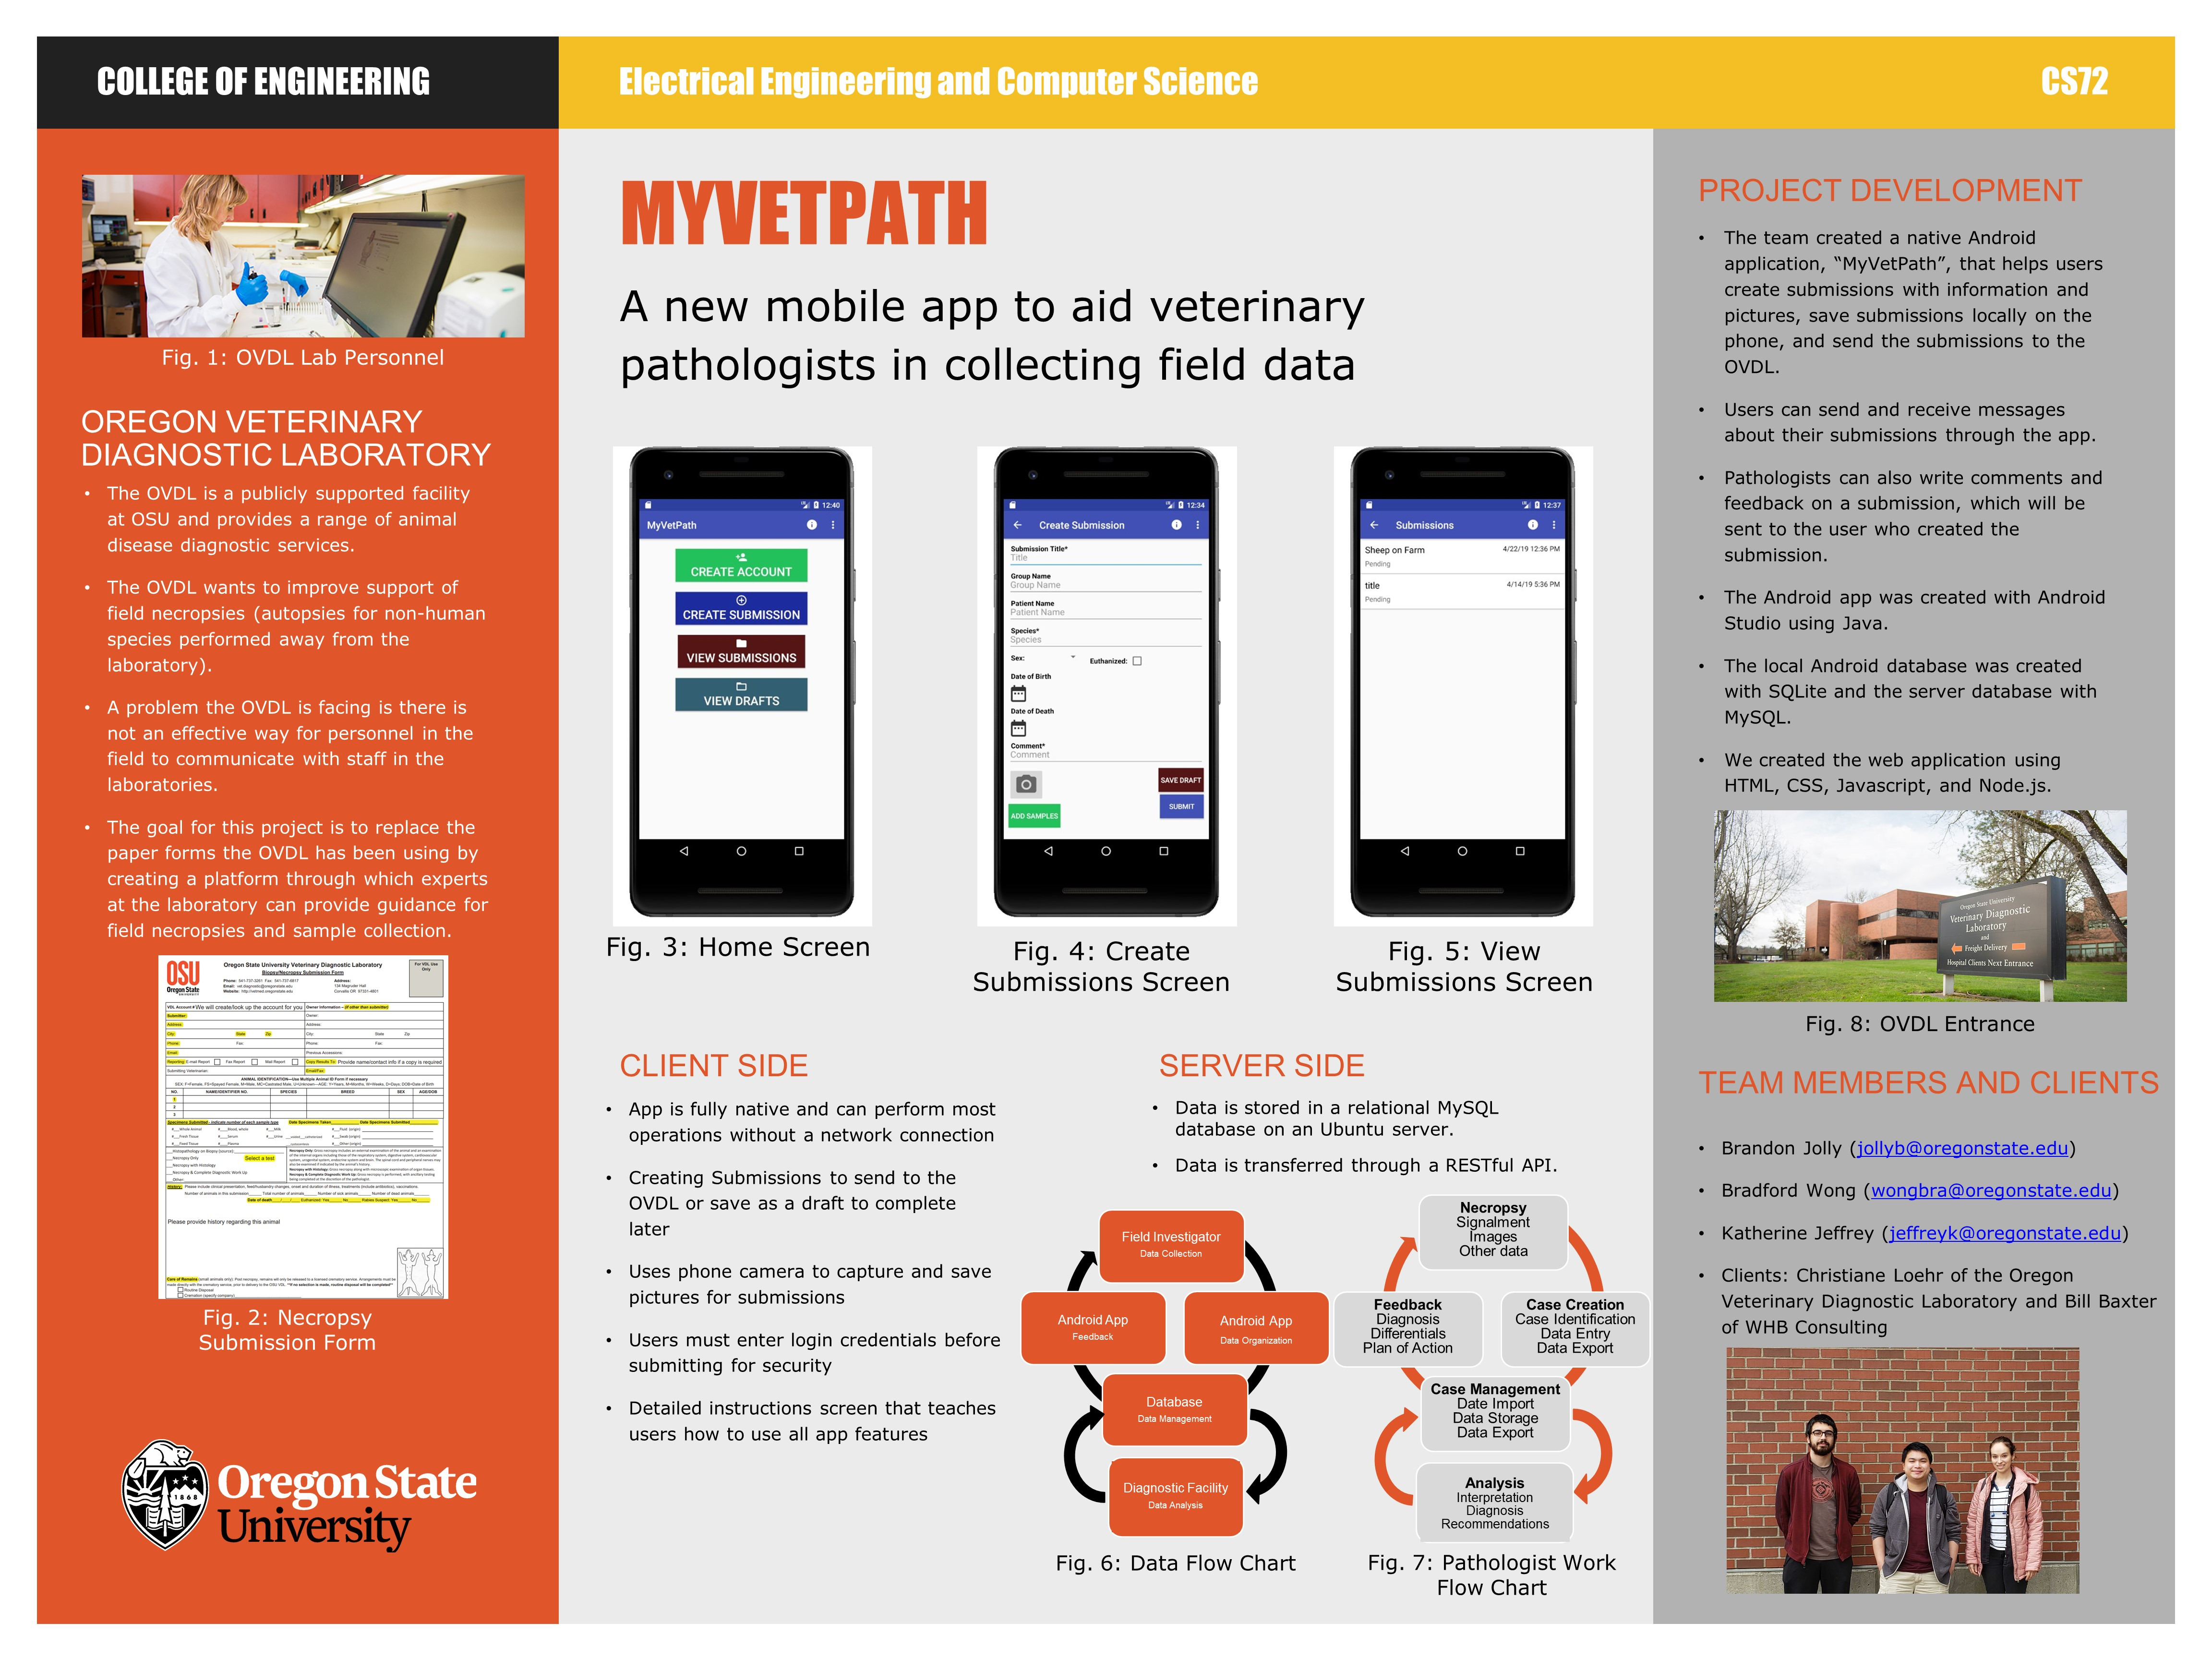
\includegraphics[height=12cm]{group72_poster_48x36.jpg}
\end{center}
\captionof{figure}{Group 72 Poster}
 
 \section{Project Documentation}
 \subsection{How Does the Project Work?}
 The project is a typical Android application. Android applications have various screens that a user can navigate to. Each screen is an activity, and an Android application is comprised of a series of linked activities. Each activity has a corresponding layout, which is a specification of what the contents of a screen should look like. All layout files can be found in the /app/src/main/res/layout/ folder. The layout files begin with "content" and then contain the name of the activity they are associated with. The activity files themselves can be found in /app/src/main/java/com/myvetpath/myvetpath, and their file names end with "Activity.java". The code in these activity files are executed at run time when the user navigates to the corresponding screen. Android activities have various predefined methods that are overriden. For example, the "onCreate" method is a predefined method that is called when the user first navigates to that screen. This method is overridden in order for the application to initialize the screen.
  
The Android application also uses a SQLite database. The tables in the SQLite database can be found in /app/src/main/java/com/myvetpath/myvetpath/data, and the name of their files always ends in "Table.java". 

Lastly, the project also uses a MySQL database. This database is saved on an Ubuntu server. An API sends data from the Android application to this server.

 \subsection{How to Install the Software}
 In order to install the software, clone the repository at https://github.com/jeffreykat/MyVetPath. Android Studio will also be necessary to develop the application, which can be found at https://developer.android.com/studio. To install Android Studio, click on the "Download Android Studio" and then run the installation wizard once it downloads. The wizard will then guide you through all of the installation steps. Once Android Studio install, you will also need to install a virtual device so that you can run the project. Click on the green "play button" at the top right and then click on the "Create New Virtual Device" button. Afterwards, select any phone on the list, click on "Next", then download a system image by clicking on "Download" next to the API you want, and then agree to the terms and download it. 
 
 \subsection{How to Run the Project}
 Open Android Studio and then open up the cloned project (go to "File -$>$ Open" and then select the cloned project). Once the project loads, there will be a green "play" button at the top right of Android Studio. Clicking on that button will open a window with a list of virtual devices that you want to run the project on. It is also possible to run the application on an actual phone by selecting that phone from the list (provided the phone is connected to the computer with a USB cable). Click on a an available device and then click on the "OK" button. The project will now run.
 
 \subsection{Hardware Requirements}
 It is recommended to have at least 8 GB of RAM when developing an Android application when using  a virtual device. While the project should run on all devices, it may run differently depending on the device and its operating system. The team did most of the testing on a phone with an API level of 27.
 
%  Todo
%  \subsection{User Guides}
 \subsection{API Documentation}
 At the time of writing this document, the API is still very incomplete. To get more information about the current status of the API, contact Bill Baxter, who is one of our clients and is the one who was developing it. The specifications of all working routes as of this moment that are relevant to the application are as follows:
 \begin{itemize}
     \item Post /users (create user). Input: {"id", "first", "last", "email", "phone", "password", "createdAt", "updatedAt"}. Output: {"message", "user", "token", "success"}
     
     \item Get /users (Return user). Input: JWT. Output: {"user": {"id", "first", "last", "email", "phone", "password", "createdAt", "updatedAt"}, "success"}. This will return the user data for a single user.
     
     \item Get /users/all (return all users). Output: {user: {"id", "first", "last", "email", "phone", "password", "createdAt", "updatedAt"}, "success"} for all users.
     
     \item Put /users (update user). Input: Any users fields except email or phone number. Output: {"message", "success"}
     
     \item Delete /users (delete user). Input: JWT, output: none.
     
     
     \item Post /users/login (User Login Authentification). Input: {email or phone number, password}. Output: { "token", "user": {id, first, last, email, phone, password, createdAt, updatedAt"}, "success"}
     
     \item Post /submissions. Input: {"submission\_id", "User\_id", "Group\_id", "Case\_id", "Title", "createdAt", "updatedAt"}.
     

 \end{itemize}
 \section{Build Instructions/User Guide}
 \subsection{Install Android App with APK}
  \begin{center}
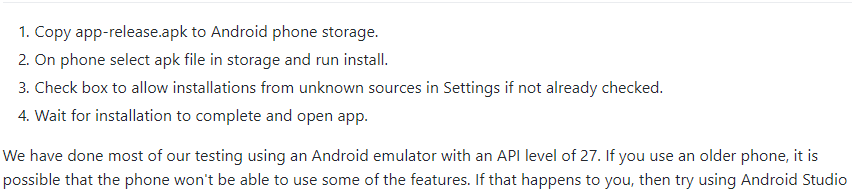
\includegraphics[height=4cm, width=18cm]{AndroidAPPScript.png}
\end{center}
\captionof{figure}{Script to install the Android App with APK}
 
\subsection{Alternative: Set Up Android Studio}
 \begin{center}
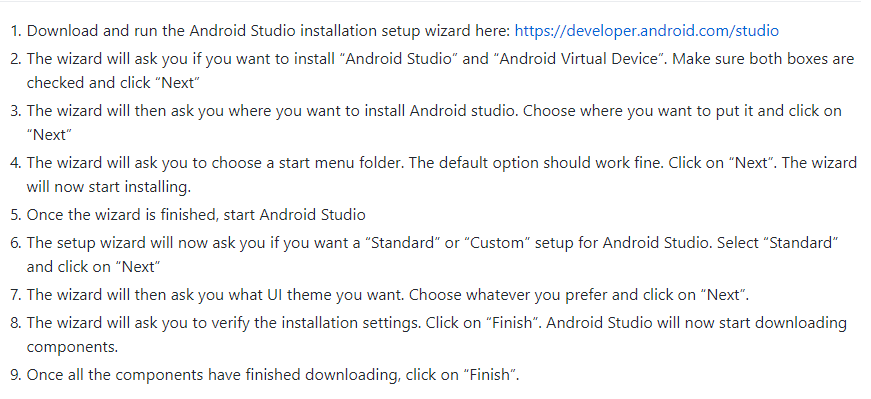
\includegraphics[height=10cm, width=18cm]{setUpAndroidStudio.png}
\end{center}
\captionof{figure}{Script to install the Android App with Android Studio}

\subsection{Clone the GitHub Repository (can be found here: https://github.com/jeffreykat/MyVetPath)}
 \begin{center}
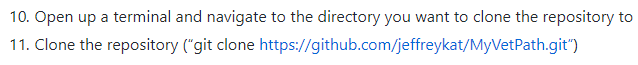
\includegraphics[height=2cm, width=18cm]{getHubClone.png}
\end{center}
\captionof{figure}{Cloning the GitHub Repo}

\subsection{Open the Project} 
\begin{center}
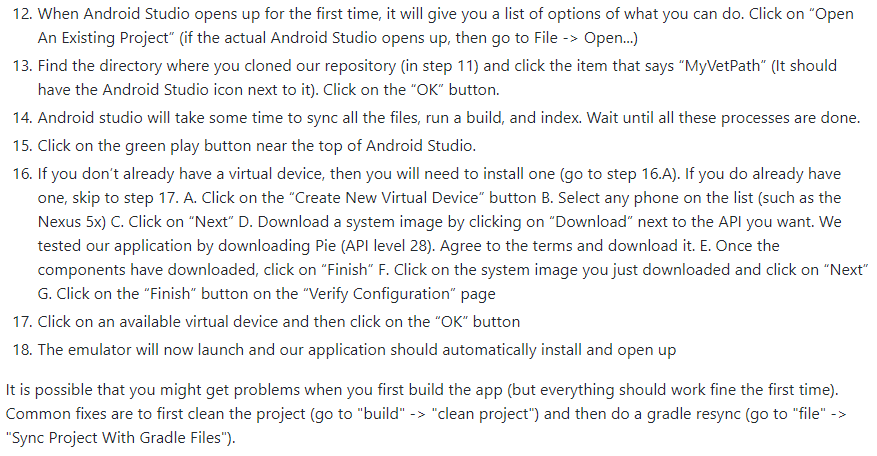
\includegraphics[height=10cm, width=18cm]{OpenProject.png}
\end{center}
\captionof{figure}{Open the ProjectScript}


\subsection{Setup MySql Server} 
\begin{center}
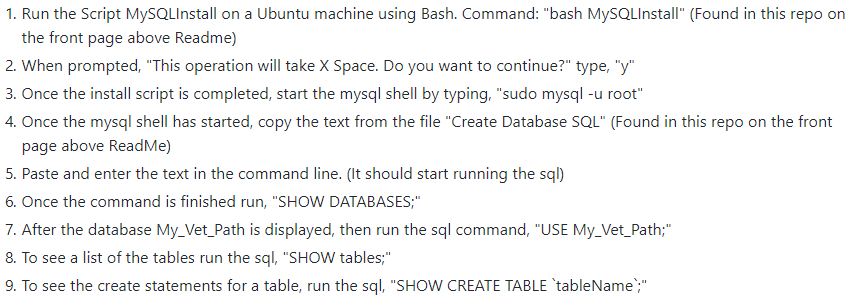
\includegraphics[height=8cm, width=18cm]{MySQLscript.PNG}
\end{center}
\captionof{figure}{Run the MySQL Script}


 \section{Recommended Technical Resources}
 \subsection{Helpful Websites}
 \begin{itemize}
     \item https://stackoverflow.com
     \item https://developer.android.com
 \end{itemize}
 
 \subsection{Helpful People on Campus}
 Rob Hess was a professor that taught a class on Android development. His lessons were very helpful to the team.
 \section{Conclusions and Reflections}
 \subsection{Brandon Jolly}
 \begin{itemize}
     \item What technical information did you learn?
     \begin{itemize}
         \item I learned how to install a database and the tables inside the database by using a Bash script. Something I have never done before. Most of the information I gained was android code. Before this takes I had not used android studio or any app development software. Over the course of this year I had gained a basic knowledge of how you develop apps and some debugging techniques.
     \end{itemize}
     \item What non-technical information did you learn?
     \begin{itemize}
         \item I learned about the process of developing a project from start to finish. Before I only knew the theory about how to create a project with a database and only then it was a rough idea. Now I had worked on a project from start to finish. Something I hadn't done in the past. 
     \end{itemize}
     \item What have you learned about project work?
     \begin{itemize}
         \item Working with a properly document design document could solve a lot of later issues. For example with our group their was some confusion on what data types to used for storing images. In our planing stage we had all of the other data types pinned down, which allowed us to implement them early on in the process. After a group meeting we were able to solve the picture issue, but it was something we could have planned for earlier.
     \end{itemize}
     \item What have you learned about project management?
     \begin{itemize}
         \item If we have a schedule written out it helps with the timing of tasks. By doing this we were able to meet our goals for the project, and it allowed us to not go over board with the features.
     \end{itemize}
     \item What have you learned about working in teams?
     \begin{itemize}
         \item Communication can solve a lot of issues. There was not really any ambiguity in who was assigned a task. Another important thing I learned was do not be afraid to ask for help. The team wants to succeed and asking for help is not shame full. In fact, it actually makes the product better for it.
     \end{itemize}
     \item If you could do it all over, what would you do differently?
     \begin{itemize}
         \item I think including the client in some more meetings would have solved a lot of headaches. During the end of winter term one of our functions was not working and we had failed to communicate to the client when our winter term deadline was. He didn't know we had one so he was working on other projects. Once we informed him we were able to get some work done but it was only a partial of the end goal.
     \end{itemize}
 \end{itemize}
  \subsection{Katherine Jeffrey}
 \begin{itemize}
     \item What technical information did you learn?
     \begin{itemize}
         \item I furthered my knowledge of Android development including SQLite databases, the Room persistence library, API level differences, and new UI features. I also learned about setting up a server. 
     \end{itemize}
     \item What non-technical information did you learn?
     \begin{itemize}
         \item I learned about the Oregon Veterinary Diagnostics Lab and they work they do there. I had not heard of it before this project. The lab and the staff there provide important services for the community and the world and I was happy to help them on this project. 
     \end{itemize}
     \item What have you learned about project work?
     \begin{itemize}
         \item It's important to have clear goals for the project from the beginning. The people working on the project should know what they are responsible for at all times and be aware of the time constraints on the project. Having a consistent method of communication between all people on the project is also important. 
     \end{itemize}
     \item What have you learned about project management?
     \begin{itemize}
         \item It's good to make detailed plans and create a schedule early. Then the team needs to stick to the schedule, but also expect delays. Feature creep is a real problem and it's best to put a stop to it early by clearly defining the project requirements and being aware of how much time the work will take. 
     \end{itemize}
     \item What have you learned about working in teams?
     \begin{itemize}
         \item This team was excellent at communicating and participating which is essential for a team to function effectively. The team was also able to work democratically, no member tried to enforce their ideas over an other's. If this had not been the case it would have been helpful to have conflict resolution strategies agreed upon in advance. 
     \end{itemize}
     \item If you could do it all over, what would you do differently?
     \begin{itemize}
         \item I would have asked for more information from the clients sooner to inform the design process early on. Too many important decisions were made late in the year and this could have been avoided if we had a better understanding of what the clients wanted from the start. It also would have been helpful to have a larger team because there was a substantial amount of work to be done and we could have delivered a much better product with more people working on it. 
     \end{itemize}
 \end{itemize}
  \subsection{Bradford Wong}
 \begin{itemize}
     \item What technical information did you learn?
     \begin{itemize}
         \item I learned a lot about how to make an Android application. For example, I learned about activities and the activity lifestyle, various ways of laying out the UI on the screen, user preferences, working with XML files, using image assets, how to work with a SQLite database, and how to use the camera and gallery to get pictures. Additionally, I learned how to use Android Studio's debugger to find and fix bugs. I also learned about APIs. I learned about what they were and how to make API requests through Postman and an Android application. I learned about how to use Retrofit, an HTTP client, to specify a request's header and body in order to make an API request in the Android application.
     \end{itemize}
     \item What non-technical information did you learn?
     \begin{itemize}
         \item I learned a lot about how to effectively communicate information. For example, I got better at communicating with my teammates and clients as time went on. I also learned about how to create documentation for a project. For example, I learned about how to write a design document and how to effectively explain the design of a software project. 
     \end{itemize}
     \item What have you learned about project work?
     \begin{itemize}
         \item I learned about working with multiple branches and how to resolve merge conflicts. I also learned about the importance of thinking about edge cases and potential ways to make the project crash. I learned this because some bugs went unnoticed for a while since we weren't thorough enough in our testing. If we were more thorough and thoughtful during testing, then we would have reduced the number of bugs in the project.
     \end{itemize}
     \item What have you learned about project management?
     \begin{itemize}
         \item I learned about the importance of carefully planning the project and always trying to think about the future. It is important to think about how certain tasks might be blocked until other tasks are completed first. As a result, we had to think about which tasks needed to be completed first. I also learned about how there can be many unexpected issues that occur during the development process. For instance, setting up the server took us much longer than we expected. As a result, I learned that you have to be flexible during the development process and be ready to work on other tasks that weren't originally assigned to you during the sprint planning meeting. Lastly, I learned about how easily feature creep can be introduced during the development process and how to deal with it.
     \end{itemize}
     \item What have you learned about working in teams?
     \begin{itemize}
         \item I learned about how often merge conflicts happen and how to effectively resolve them. I also learned the importance of writing lots of comments, because there were times when people had difficulty understanding the code that a different teammate wrote. In addition, I learned about how important good communication is in general, because there were also times when team members were confused when they saw changes to the application that weren't communicated to them.
     \end{itemize}
     \item If you could do it all over, what would you do differently?
     \begin{itemize}
         \item I would definitely start testing with actual phones sooner. We didn't start testing with actual phones until spring term, and we found numerous bugs that existed on the phones but couldn't be replicated on the emulator. As a result, we had to spend a lot of time fixing those bugs before the Engineering Expo. I would also try to be more careful about feature creep. The client and team kept coming up with new ideas for the project, but it was unrealistic to think that we could develop all of these new features within our time frame. I would make sure that the client and team both understand what the expectations for the project are and what can be reasonably be done within the time frame. 
     \end{itemize}
 \end{itemize}
 \section{Appendix 1: Essential Code Listings}
 
 \begin{center}
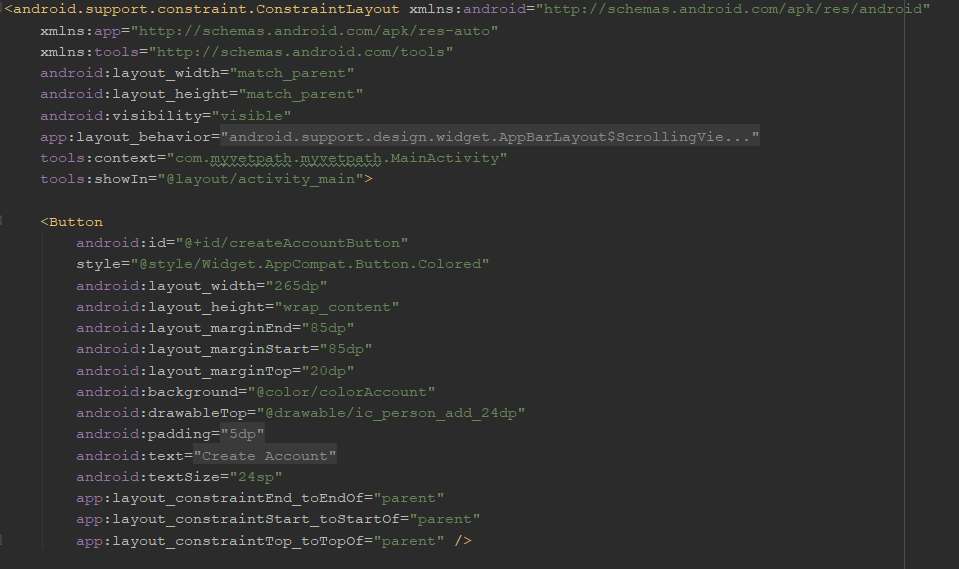
\includegraphics[height=8cm]{main_content_xml.png}
\end{center}
\captionof{figure}{XML File of Main Activity (Home Screen)}
The figure above shows the code that is used to create the Home Screen. The XML file is where the struture and layout of that screen can be specified. For example, in this code snippet, the layout specifies a button object. Each of these objects have various properties such as the width, height, text, and textSize, which can all be specified in the XML file. It is important to note that each object placed in the XML file should have an id because they are necessary to make any modifications to the objects in the Java code. It is also important to note that the screen in this example uses a Constraint Layout. Layouts specify the structure of the screen and are a way of positioning certain objects. Constraint Layouts involve specifying the constraints of an object in order to position that object. An object's position in a Constraint Layout can be specified by saying where that object is relative to another object.

 \begin{center}
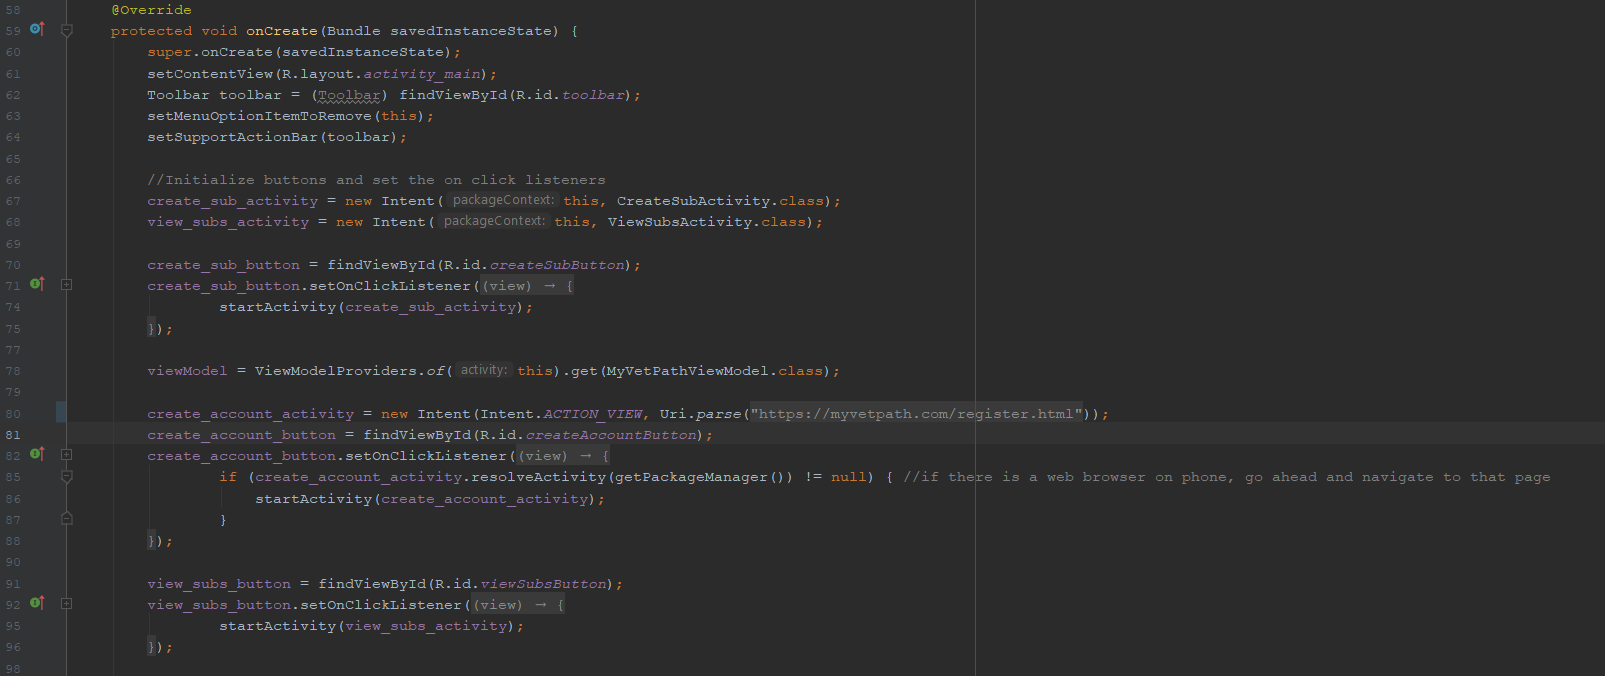
\includegraphics[height=8cm]{main_oncreate.png}
\end{center}
\captionof{figure}{Main Activity's onCreate Code}
The code snippet above is the Java code for the Main Activity, which represents the home screen of the application. The onCreate function is an essential method in all Android activities because this is is the method that initializes the screen its variables. For example, the code snippet above shows the toolbar being initialized in lines 62-64. Additionally, the snippet shows how to implement navigation within an Android application. Line 68 initializes an intent that will navigate to the ViewSubsActivity screen. On line 91, the code finds the view\_subs\_button that was created in Main Activity's XML file. Line 92 assigns an onClickListener to the button, meaning that the code inside of that block of code is executed anytime a user clicks on the button. In this case, the only code that is executed is the code in line 95, which is what will actually navigate the user to the ViewSubsActivity screen.

 \begin{center}
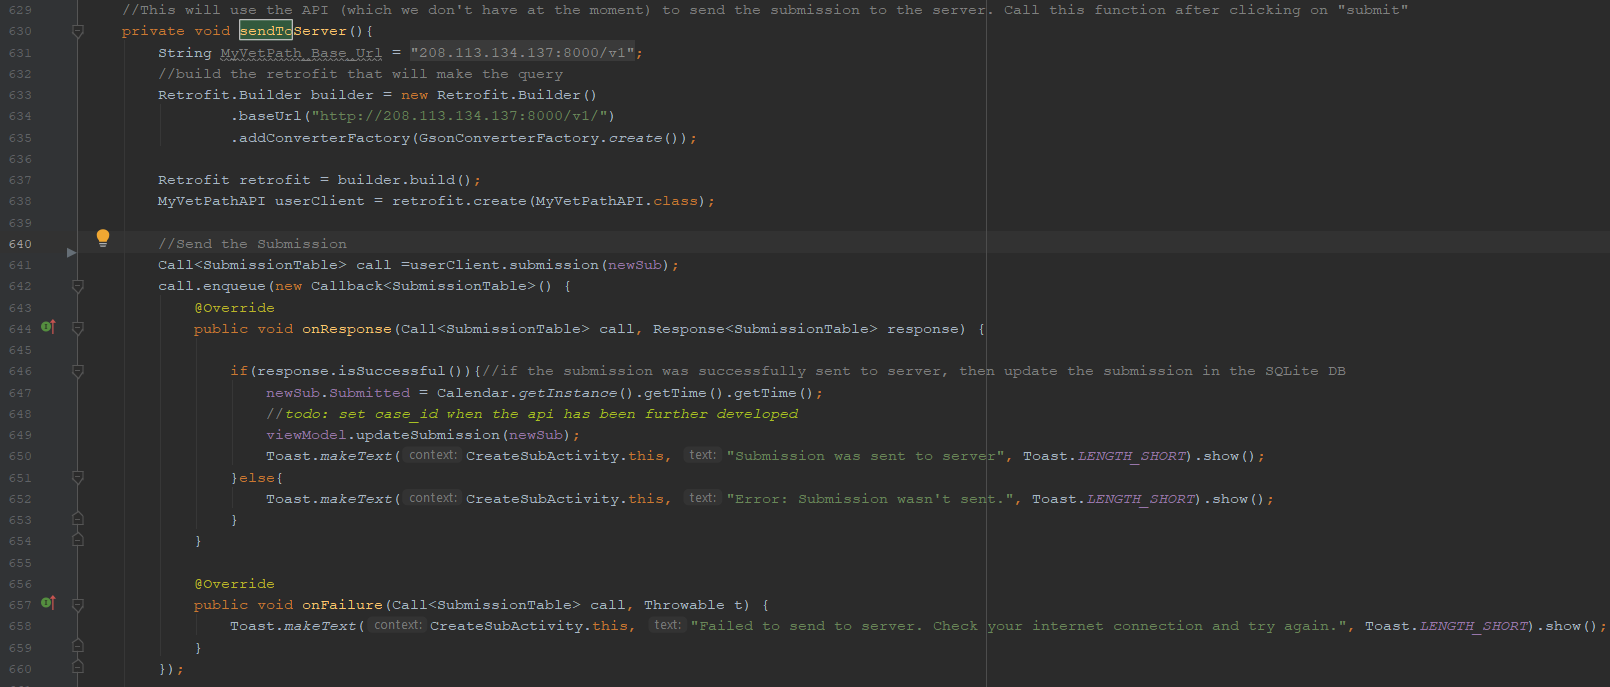
\includegraphics[height=8cm]{sendtoserverfunction.png}
\end{center}
\captionof{figure}{Code that Makes a POST Request Using the API}
The code above shows how to send a submission to the server's database by making a POST request. The Android application uses Retrofit, which is an HTTP client that is used to make API requests. The code in lines 631-638 sets up Retrofit. Lines 641-660 is the code that actually sends the submission to the server. The onResponse method is called after getting a response back from the server. If the response was successful, then the application will update the submission and display a message to the user saying that submission was sent successfully. If the server sent an error back, then the application will just display an error message instead. The application can receive a failure response if something was wrong about the API call. For example, if the POST request went to the wrong route, the Bearer Token was incorrect, or if server was expecting a different body of data. The API is what sends these failure responses. the onFailure method is called whenever the application fails to make the API request and doesn't get a response from the server. This typically happens when the server isn't down or if the user isn't connected to the internet.

\begin{center}
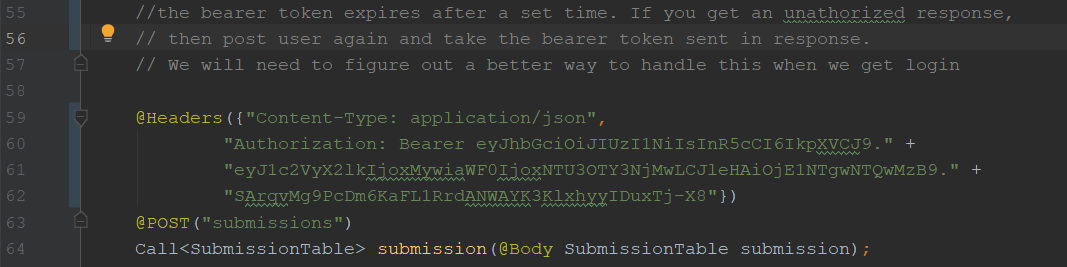
\includegraphics[height=5cm, width=18cm]{api_call_fixed.png}
\end{center}
\captionof{figure}{Code that Defines the API Request}
The code above shows how to specify a POST reqest using the API. The header should always have "application/json" as the content-type. The authorization is the Bearer Token that is assigned whenever a user is created. The "submissions" part following the "@Post" part is the route. Finally, the body of the API call is just the class that is being sent to the server, which is "SubmissionTable" in this example.

\begin{center}
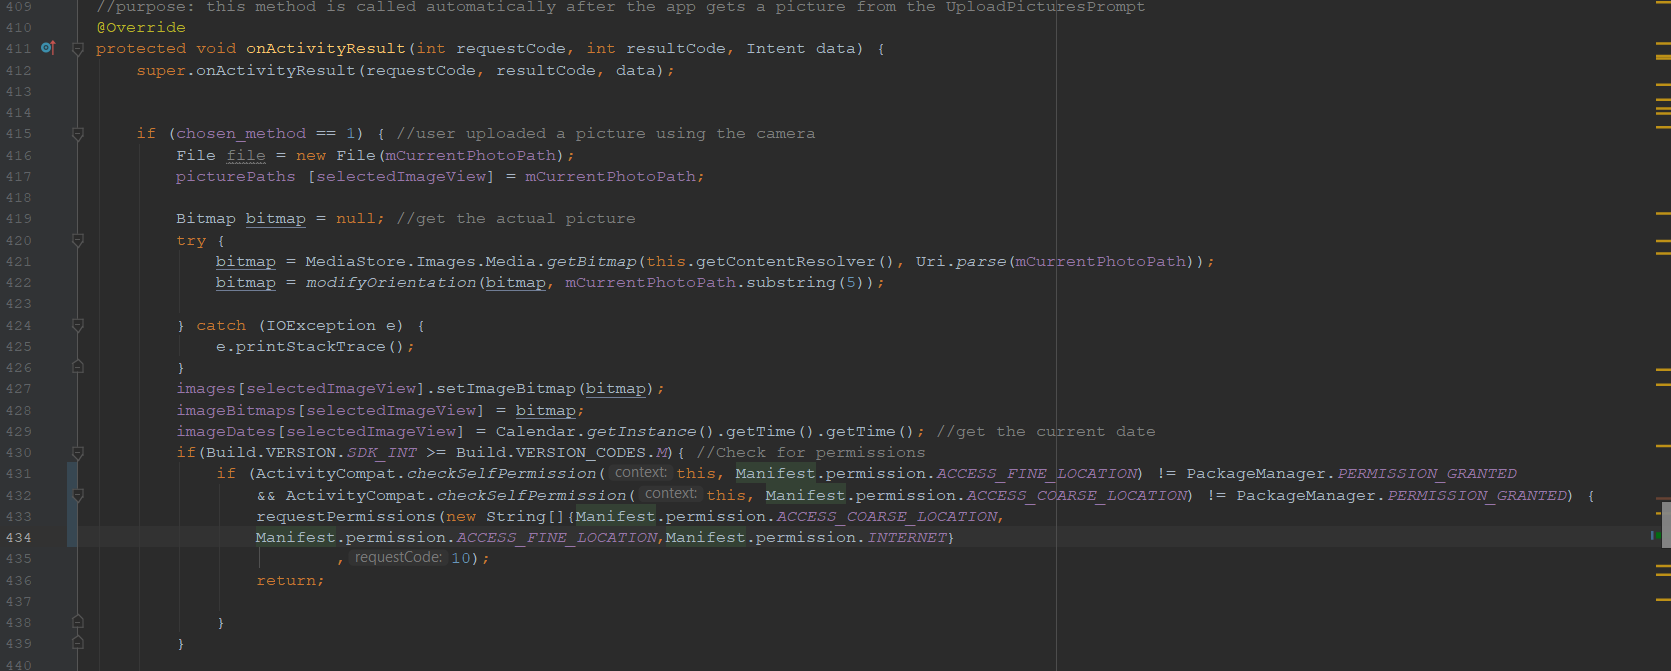
\includegraphics[height=8cm, width=18cm]{onactivityresults1.png}
\end{center}
\captionof{figure}{Code that Gets a Picture (Part 1)}


\begin{center}
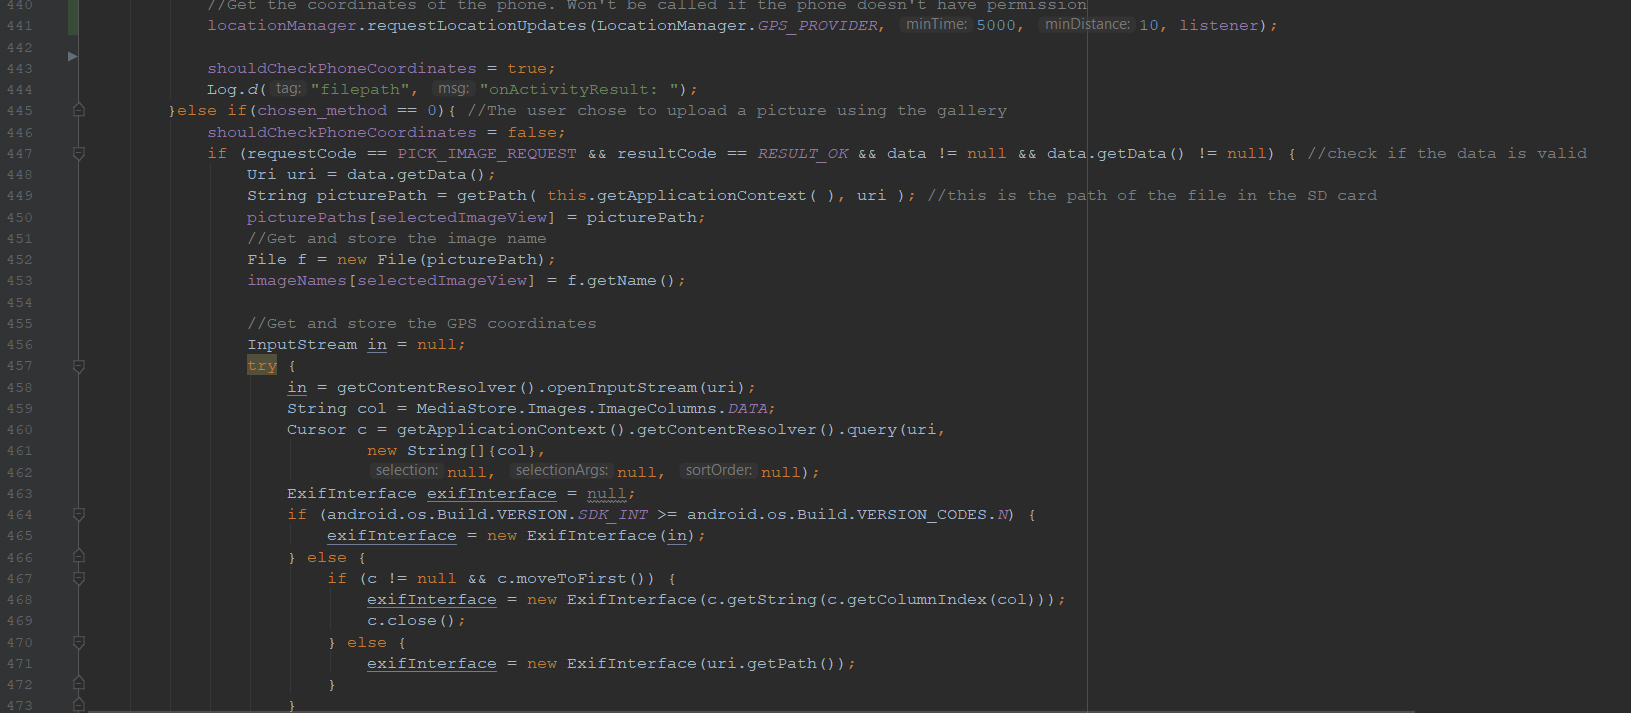
\includegraphics[height=8cm]{onactivityresults12.png}
\end{center}
\captionof{figure}{Code that Gets a Picture (Part 2)}

\begin{center}
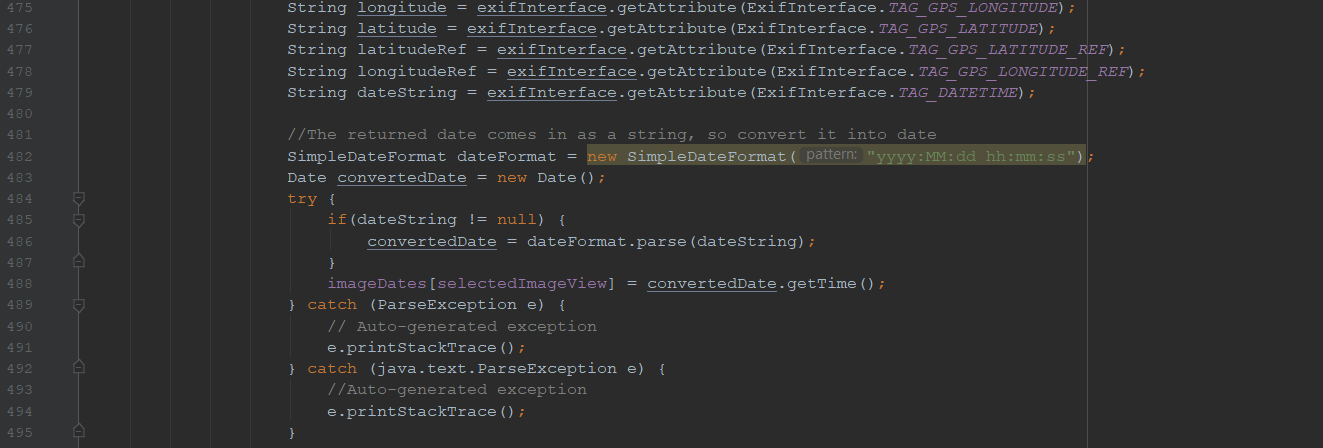
\includegraphics[height=8cm, width=18cm]{onactivityresults3.png}
\end{center}
\captionof{figure}{Code that Gets a Picture (Part 3)}

\begin{center}
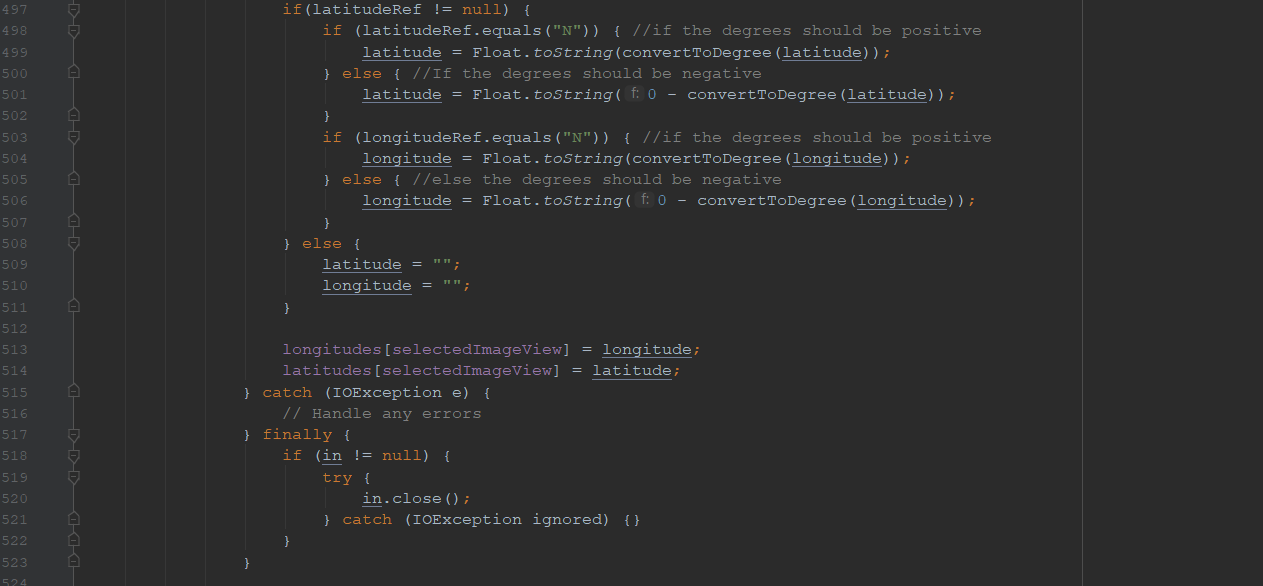
\includegraphics[height=8cm]{onactivityresults4.png}
\end{center}
\captionof{figure}{Code that Gets a Picture (Part 4)}

\begin{center}
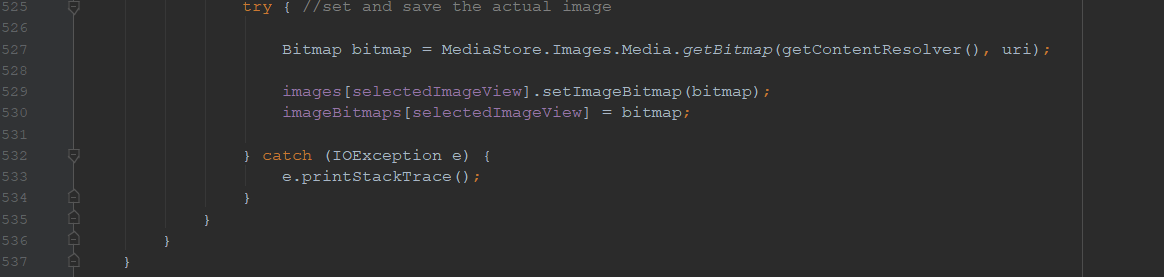
\includegraphics[height=5cm, width=18cm]{onactivityresults5.png}
\end{center}
\captionof{figure}{Code that Gets a Picture (Part 5)}
The five figures above show a picture is obtained in the "AddPicturesActivity" screen. This method is called automatically whenever the user selects a picture from gallery or takes a picture from the camera. If the user took a picture with the camera, then the application will execute lines 416-444. Lines 416-426 is what gets the actual picture and stores it into a bitmap. Some phones have an issue where taking a picture automatically rotates or flips it. To deal with this, line 422 calls a function that simply rotates it back to normal. Lines 427-428 saves the picture into the variables in the class, which will actually display the picture on the screen. Lines 429-444 obtains the metadata of the picture such as GPS coordinates and the time it was taken. Lines 430-435 checks to see if the phone has permission to get the location metadata.

If the user selected a picture from the gallery, then the code from lines 446-536 will be called. The application first checks to see if it has permission and if the data that came back is valid in line 447. Lines 448-453 is what gets the picture. Lines 456-523 is where the application tries to get the metadata of the picture. Finally, lines 525-534 gets the bitmap of the picture and saves it into the class' variables.

 \section{Appendix 2}
 
 \bibliographystyle{IEEEtran}
\bibliography{refs}
\end{document}








